\documentclass[msc,numbers]{coppe}
\usepackage[utf8]{inputenc}
\usepackage{amsmath,amssymb}
\usepackage{hyperref}
\usepackage[inline]{enumitem}
\usepackage{subfig}

\makelosymbols
\makeloabbreviations

\begin{document}
  \title{Análise de Sentimento em Redes Sociais por Classificadores Multimodais de Aprendizado de Máquina}
  \foreigntitle{Sentiment Analysis on Social Networks by Multimodal Machine Learning Classifiers}
  \author{Breno}{Vieira Arosa}
  \advisor{Prof.}{Luiz}{Pereira Calôba}{Dr.Ing.}
  \advisor{}{Natanael}{Nunes de Moura Junior}{D.Sc.}

  \examiner{Prof.}{Luiz Pereira Calôba}{Dr.Ing.}
  \examiner{}{Natanael Nunes de Moura Junior}{D.Sc.}
  \examiner{Prof.}{Nome do Terceiro Examinador Sobrenome}{D.Sc.}
  \examiner{Prof.}{Nome do Quarto Examinador Sobrenome}{Ph.D.}
  \examiner{Prof.}{Nome do Quinto Examinador Sobrenome}{Ph.D.}
  \department{PEE}
  \date{09}{2019}

  \keyword{Análise de sentimento}
  \keyword{Processamento de linguagem natural}
  \keyword{Redes complexas}
  \keyword{Aprendizado de máquina}

  \maketitle

  \frontmatter
  \dedication{A algu\'em cujo valor \'e digno desta dedicat\'oria.}


  %\chapter*{Agradecimentos}

Muitas foram as pessoas que me permitiram concluir este trabalho.
À todas elas deixo aqui os meus agradecimentos.

A UFRJ está presente em minha vida ao longo dos últimos 11 anos.
Pensar na instituição é, em essência, lembrar de todos que estiveram presentes nesse período.
Foram incontáveis as pessoas incríveis que aqui conheci.
Os funcionários e professores com quem tanto aprendi.
Os integrantes do LPS, que propiciaram experiências de vida inesquecíveis no CERN e um currículo profissional distinto.
Especialmente todos que dividiram comigo os encontros de corredor, as horas nas bibliotecas, as refeições e tantos outros momentos que passei neste lugar e me renderam amigos e amores.
À esta universidade dedico um agradecimento profundo.

Estas páginas marcam o fim de uma etapa e proporcionam o florescimento de novas.
Estarão comigo todos os que fizeram parte do caminho.

  \begin{abstract}

Nos últimos anos, as redes sociais se tornaram um dos principais meios de
comunicação, e com isso, houve um aumento da influência que exercem sobre os
usuários.
Por esse motivo, as mensagens que trafegam por elas passam a ter importância
para as mais diversas finalidades como, por exemplo, a avaliação de produtos e
eventos.
Dessa forma, esse tipo de texto se faz passível de diversas análises, sendo a
mineração de opinião é uma das operações com mais aplicações diretas.
Nesse sentido, ferramentas de processamento de linguagem natural e de redes
complexas são capazes de auxiliar a geração destas análises.
Entretanto, o desempenho dessas técnicas, em geral, depende da existência e do
volume de bases de treinamento anotadas manualmente, dificultando assim a sua
utilização.
O presente trabalho aplica métodos de geração de bases de treinamento
automatizadas para contornar tal obstaculo e gerar classificadores de análise
de sentimento.
São avaliados diferentes modelos de classificação textual, tanto lineares,
como Naïve Bayes e SVM, quanto não lineares, como por \textit{Deep Learning}.
Também são analisadas técnicas de redes complexas para caracterização dos
usuários das redes, abordando, assim, diferentes aspectos das informações
fornecidas por estas mídias.

\end{abstract}

  \begin{foreignabstract}

During the last years, social media became one of the main communication channels, growing its influence over its users.
Accordingly, the messages that run on social media started to be relevant for a wide range of applications, such as product reviews.
Consequently, initiating a variety of analyses on this modality of text, one of them being the sentiment analysis which has clear direct applications.
In this manner, techniques of natural language processing and complex networks can assist in these analyses.
However, the performance of these tools usually depends on the volume of manually labeled training data, therefore adding costs to its utilization.
This work applies a method of automatic data labeling to generate training datasets and avoid this barrier.
Multiple text classification models are evaluated, both linear and non-linear, such as Deep Learning.
Additionally, we assess complex network techniques on the task of representing users.
Therefore, multiple aspects of the information available on these social networks are considered by the models.
The experiments ran by this work demonstrate that for the collected social media dataset,
linear methods were superior than the neural network models, reaching $0.801$ AUC.
Additionally, contrary to expectations, it was also observed that the information present on the users network formed by republishing posts wasn't sufficient to improve the sentiment analysis results.

\end{foreignabstract}


  \tableofcontents
  \listoffigures
  \listoftables
  \printlosymbols
  \printloabbreviations

  \mainmatter
  \chapter{Introdução}
\label{chapter:intro}

Nas últimas duas décadas, as redes sociais se tornaram um dos principais meios de
comunicação.
Esse crescimento se justifica, em parte, pela massificação do acesso a internet,
proporcionada em grande medida por dispositivos móveis como \textit{smartphones}
e \textit{tablets}.
Também alavancado pelos avanços computacionais e pelo desenvolvimento acelerado
de novas técnicas e algoritmos, o aprendizado de máquina, em especial o
processamento de linguagem natural, tem essas redes como importante objeto de
estudo.

Desde a chamada Revolução Digital, observamos um progressivo barateamento e
facilitação do uso de dispositivos eletrônicos.
À medida que essas tecnologias passaram a ser acessíveis, não apenas para as
corporações, mas também para os indivíduos, houve um crescente processo de
digitalização de diversos aspectos de nossas vidas.
Com a comunicação não foi diferente.
O email, por exemplo, substitui desde os anos 70 operações que até então eram
apenas possíveis de forma analógica, como pelo uso de cartas.
Nesse contexto, as redes sociais, ou mídias sociais, abordam aspectos diferentes
da comunicação, mais dinâmica e informal.

Apesar de já existirem desde os anos 90, é com a virada do milênio que as
primeiras grandes mídias sociais online aparecem, como \textit{LinkedIn},
\textit{MySpace} e \textit{Orkut}.
Desde então há um aumento anual da quantidade de seus usuários.
Atualmente, estima-se que 3,5 bilhões de pessoas, isto é, 45\% da população mundial
utilize pelo menos uma rede social.
Este número torna-se ainda mais interessante quando considerado que 4,4 bilhões
de pessoas têm acesso à internet.
Portanto, quase 80\% dos internautas estão em alguma das mídias sociais.
No Brasil, esses números se acentuam ainda mais: 70\% da população tem
acesso à internet e 66\% utiliza as redes sociais~\cite{social19}.

Além da alta penetração na sociedade, devido à disponibilidade proporcionada
pelos dispositivos móveis, os usuários consomem boa parte de seu tempo nessas
redes.
No mundo, gasta-se em média 2 horas e 16 minutos por dia.
Novamente, esse número é ainda superior no Brasil, onde a média é de 3 horas e
34 minutos, caracterizando-se como segundo país no mundo a usar por mais tempo
as redes, atrás somente das Filipinas~\cite{social19}.

Essa forte presença fez com que as mídias sociais não impactassem apenas as
comunicações.
Hoje em dia, esses meios também são comumente utilizados para buscas de
relacionamentos, compartilhamento de notícias, divulgação de serviços,
atendimento ao público, entre outros~\cite{mangold09}.
As informações que trafegam nas redes exercem grande influência na formação de
opinião das pessoas, seja em relação a um produto, a um evento ou até mesmo
a temas políticos, como pôde-se observar em eleições pelo mundo nos últimos anos.

Portanto, a análise de tais informações, presentes nas redes, é importante para
as mais diversas aplicações.
Contudo, essa grande quantidade de usuários também se reflete no número de dados
provindos das mídias sociais.
Dentre as estatísticas de uso do ano de 2018 fornecidas pelas próprias redes
sociais, tem-se que, diariamente, 300 milhões de fotos são publicadas no
\textit{Facebook}, 5 bilhões de vídeos são vistos no \textit{YouTube}, 43
bilhões de mensagens são enviadas no \textit{WhatsApp} e 100 milhões de usuários
interagem pelo \textit{Twitter}.
% dados de https://dustinstout.com/social-media-statistics/

O massivo volume de dados inviabiliza que essas análises sejam feitas
manualmente, tornando-se necessário o desenvolvimento de ferramentas capazes de
automatizar esse processo.
Faz-se necessária a aplicação de técnicas desenvolvidas pelo campo do
Processamento de Linguagem Natural, do inglês \textit{Natural Language Processing}
(NLP)\abbrev{NLP}{Natural Language Processing}.
Foi a partir do anos 50 que esse termo passou a aparecer como um ramo da
Inteligência Artificial~\cite{hutchins04}.
Devido à sua complexidade, a linguagem natural acabou inclusive se tornando um
critério de inteligência, como proposto no teste de Turing~\cite{turing50}.

O NLP é uma ampla área de pesquisa, abrangendo diferentes estágios da língua,
desde os níveis de abstração mais baixos, como o estudo da fonologia e da
sintaxe, até os níveis de abstração mais altos, que lidam com a semântica de
determinado conteúdo~\cite{nadkarni11}.
Nesse ramo, busca-se desenvolver métodos capazes de auxiliar e/ou automatizar
tarefas como o reconhecimento de fala, a análise sintática de frases, a
extração de entidades, a segmentação por tópicos, entre outros~\cite{hirschberg15}.
Esse conjunto de ferramentas é essencial para tratar o volume de textos
gerado pelas redes sociais.

Com o avanço de técnicas de \textit{Deep Learning}, nos últimos anos pôde-se
observar uma melhora significativa de desempenho, que permitiu a realização mesmo
de tarefas de grande dificuldade, como a automatização de traduções e de aplicações
de atendimento ao cliente por conversação~\cite{hirschberg15}.
Entretanto, apesar do grande potencial dessas técnicas, as mídias sociais
apresentam características que diferenciam seu conteúdo dos gêneros textuais que
tradicionalmente se analisam em NLP, como artigos científicos e textos
jornalísticos, dificultando o processamento dessa informação.
Em geral, as redes sociais se apresentam como um meio de conversação ágil, logo,
as mensagem que circulam por elas costumam ser extremamente curtas, com amplo
uso de abreviações.
Por seu caráter informal, observa-se uma alta taxa de erros gramaticais e
uma grande utilização de \textit{emoticons}~\footnote{Sequência de caracteres ou
pequena imagem que transmite um estado emotivo}.
Somado a isso, o fato de serem meios de comunicação globais também ressalta a
presença de estrangeirismos~\footnote{Uso de palavras ou expressões estrangeiras}.
Ademais, a dinamicidade das redes sociais faz com que a evolução do sentido das
palavras seja acelerada.
Esses elementos trazem a necessidade de adaptação ou desenvolvimento de novas
técnicas para se reproduzir o sucesso obtido pelas técnicas de processamento de
texto em documentos com escrita mais formal e estruturada.

No entanto, o principal fator que distingue as informações de redes de outros
meios é a forte interligação entre diferentes tipos de mídia, como textos, imagens,
áudios, fotos e vídeos.
Além de metadados importantes, como localização, data e horário, uma propriedade
relevante das mídias sociais são os atributos referentes às redes de usuário.
Exemplos desses dados são o número de amizades de um usuário da rede e o
número de re-compartilhamentos de uma mensagem.
Logo, apesar da capacidade das ferramentas de NLP, existe um conjunto de
informações que essas técnicas desconsideram, abrindo espaço para que as
abordagens multimodais, ou seja, que explorem diversas destas propriedades,
explorem esses elementos complementares.

As interações entre usuários são o cerne das mídias sociais.
Logo, técnicas que se dispõem a analisar esse tipo de informação também são de
grande relevância.
Nesse quesito, o campo das Redes Complexas, também chamado de Ciência de Redes,
é responsável por estudar os algoritmos e comportamentos observados em grafos
que representam sistemas reais, como no caso das redes sociais.
Assim como o aprendizado de máquina, essa esfera do conhecimento também
demonstra um grande crescimento nos últimos anos, fornecendo um novo leque de
tecnologias, de forma a descobrir aplicabilidades até então inexploradas.
Dentre suas aplicações, que possuem importância para o estudos das mídias
sociais, pode-se ressaltar, por exemplo, a detecção de comunidades, a
identificação de principais influenciadores e a modelagem de propagação de
informação~\cite{barabasi16}.

Finalmente, esses métodos são poderosas ferramentas de análise das redes sociais,
principalmente quando aplicados em complemento à informação textual.
A complementariedade entre os métodos em questão permite, por exemplo, distinguir
conotações de uma mesma mensagem quando escritas por usuários de comunidades de
ideias opostas.
Por conta de casos complexos como esse, nos quais a análise de um único elemento
da mensagem não é suficiente para sua classificação, se fazem necessários
estudos que contemplem a multimodalidade das redes sociais.

\section{Motivação}

Dados são considerados um dos bens mais valiosos da atualidade, de forma mesmo a
serem chamados de ``o novo petróleo''.
Isso porque, assim como o petróleo, os dados são preciosos e precisam ser refinados
para terem utilidade.
Um dos aspectos dessa transformação pode ser observado na mudança cultural de
organizações e empresas que passam a tomar decisões baseadas em dados e métricas
coletados.

A busca por informação de qualidade sobre um serviço ou produto sempre foi
importante para consumidores.
Quando não havia as tecnologias utilizadas atualmente, essas pesquisas eram feitas
majoritariamente pelo boca-a-boca ou a partir de revistas especializadas.
Com a criação da internet e das redes sociais, estas passaram também a exercer
essa função, pelo beneficio de se encontrar opiniões de forma espontânea e em
grande quantidade.
As empresas, por sua vez, têm a oportunidade de utilizar as opiniões que
trafegam nas redes para identificar falhas em suas mercadorias, melhorar sua
segmentação, planejar novos produtos, entre outras atividades.
Com o fácil acesso à coleta desses dados, as ferramentas capazes de extrair o
sentimento dessas mensagens tornam-se fundamentais para viabilizar esse
procedimento na escala em que elas ocorrem.

Apesar das dificuldades inerentes à classificação de dados não estruturados,
técnicas de aprendizado de máquina, sobretudo \textit{Deep Learning}, e de Redes
Complexas apresentam, ao longo dos últimos anos, melhorias de performance em várias
tarefas realizadas sobre mensagens de redes sociais.
Entretanto, o desempenho desses modelos depende, em geral, da quantidade de dados
anotados disponíveis para treinamento.
Como o processo de anotação é manual, esse passa a ser o gargalo da construção de
classificadores de sentimento.

Tal empecilho se torna ainda mais notável quando consideram-se aplicações que
requerem a análise de diferentes línguas ou que tenham foco em um tema
específico, necessitando criação de bases de dados próprias para cada caso de
uso.
Estes fatos motivam a elaboração de métodos que sejam independentes de bases de
treinamento.

\section{Objetivo}

Este projeto visa a desenvolver um método capaz de formar classificadores de
análise de sentimento sem a necessidade anotação de bases de dados de treinamento.
A análise será feita sobre dados de mídia sociais, explorando tanto a mensagem textual
contída nas publicações, quanto informação obtida a partir das redes de usuários.
A principal meta deste trabalho é viabilizar o emprego de modelos complexos,
que se beneficiam de um grande volume de dados, sem o custo proveniente da anotação
de bases.

Para a análise das mensagens será avaliado o impacto da utilização de
classificadores baseados em modelos de \textit{Deep Learning} em comparação a
métodos lineares tradicionalmente aplicados em NLP.
Diferentes estratégias de representação de palavras e arquiteturas de
classificadores de redes de aprendizado profundo serão testadas de acordo com o
estado da arte em processamento de texto.
O treinamo dos modelos será feito de maneira semi-supervisionada com supervisão distante,
para anotação automática dos dados de treinamento.

Técnicas de Redes Complexas serão aplicadas para a caracterização dos autores das
mensagens.
Serão comparados modelos de representação de nós em grafos, também baseados em
aprendizado de máquina e com treinamento não supervisionado, cujo custo
computacional permita operar em volumes de dados compatíveis com os de redes
sociais.
Nesse caso, além de avaliar os modelos entre si, será analisada a informação
adicional provinda dos usuários quando aplicada em conjunto com o classificador
textual.

Por fim, há um amplo conjunto de estudo aplicando NLP em redes sociais.
Adicionalmente, a ciência de redes também tem um grande reportório de pesquisa
sobre esse meio de comunicação.
Assim, este trabalho visa a preencher a lacuna de sistemas que não necessitam de
investimento em anotação de bases e que abrangem a multimodalidade da
informação característica desse tipo de dado.

%\section{Contribuições}
\section{Organização do Texto}

Esse documento é organizado da seguinte maneira:

\begin{itemize}
    \item O Capítulo~\ref{chapter:sentiment} apresenta o problema da análise
        de sentimento aplicada em mídias sociais e os seus desafios.
        Esse capítulo contém uma breve revisão bibliográfica de classificadores
        de análise de sentimento e de técnicas de redes aplicadas à essa tarefa.
    \item No Capítulo~\ref{chapter:nlp}, as técnicas de processamento de
        linguagem natural são apresentadas.
        São caracterizadas as diferentes formas de representação numérica das
        mensagens e sobre quais premissas se baseiam.
        Também são descritos os classificadores, tanto os métodos lineares
        tradicionalmente aplicados a textos, quanto os de \textit{Deep Learning}.
    \item As ferramentas de ciência de redes são apresentadas no
        Capítulo~\ref{chapter:networks}.
        Nele, são mostradas as diferentes técnicas de representação de
        vértices de uma rede, que serão aplicadas na modelagem de usuários de
        mídias sociais.
    \item O Capítulo~\ref{chapter:method} descreve o método proposto para
        desenvolvimento dos classificadores.
        São apresentadas as etapas de formação de bases de dados, de anotação
        automática das mesmas e de sua classificação.
    \item Os resultados obtidos pelos experimentos propostos são mostrados e
        avaliados no Capítulo~\ref{chapter:results}.
    \item Por fim, o Capítulo~\ref{chapter:conclusion} apresenta as conclusões
        e enumera possíveis desdobramentos do trabalho realizado.
\end{itemize}

  \chapter{Análise de Sentimento de Redes Sociais}
\label{chapter:sentiment}

A Análise de Sentimento é o campo de estudos que analisa opinião, sentimento,
atitude e emoções de pessoas em relação a entidades.
Essas entidades podem ser outras pessoas, eventos, produtos, tópicos etc.
Na literatura, também se encontram os seguintes nomes relacionados a esse ramo:
\textit{mineração de opinião}, \textit{extração de opinião},
\textit{mineração de sentimento}, \textit{análise de subjetividade},
\textit{análise de emoção} e \textit{extração de críticas}~\cite{liu15}.
Por ser aplicado majoritariamente a textos escritos, este campo é filiado
ao processamento de linguagem natural, sendo uma de suas ramificações mais
ativas.

Segundo \citet{cambria16}, a Análise de Sentimento é dividida entre duas
principais tarefas, a extração de polaridade e a detecção de emoções.
Enquanto a primeira se concentra em discernir conteúdo positivo de negativo,
a segunda é responsável por classificar o documento em emoções como felicidade,
medo, raiva e tristeza.

A autora \citet{liu15}, por sua vez, ressalta que há diferentes níveis de
granularidade de execução desta tarefa.
A escolha do nível a ser utilizado depende da finalidade pela qual se aplicará
a classificação e será uma das principais caraterísticas para definir o tipo
de técnica empregada.
A Análise de Sentimento pode ser realizada a nível de documento, no qual um
documento, como uma avaliação de produto, é analisado como um todo.
Nesses casos, assume-se implicitamente que um documento expressa uma opinião
sobre uma única entidade, como o produto em questão no exemplo citado.
Também fica implícito que o documento expressa um sentimento único sobre a
entidade.
Por serem textos mais extensos, logo com mais informação, a assertividade de
modelos nesses casos geralmente é mais alta.
Portanto, mesmo as técnicas mais simples como as baseadas em dicionário, como
serão apresentadas na seção~\ref{sec:dictionary}, podem obter resultados
suficientemente bons.
\citet{taboada11} exemplifica a extração de opinião de documentos a partir de
técnicas de dicionário aplicadas em diferentes a bases de dados de avaliações de
produtos.
Por sua vez, \citet{das07} realiza predições de valores de ações a partir de
análise de sentimento das mensagens de um fórum online de investidores.

Visto que as limitações decorrentes de se classificar documentos por inteiro
reduzem o escopo de aplicações possíveis, pode-se recorrer ao nível seguinte de
granularidade: a classificação de sentimento de sentenças.
A principal diferença entre essa abordagem e a anterior é a quantidade de
informação disponível, dado que uma sentença é composta, geralmente, por poucas
palavras.
Por outro lado, a premissa do sentimento único no conteúdo de uma frase é mais
coerente com a realidade quando comparada com a classificação do documento como um
todo, sendo uma aproximação suficientemente boa para uma nova gama de casos de uso.
Entretanto, \citet{liu15} ressalta que para o caso de sentenças é importante que
a classificação de polaridade leve em consideração o sentimento neutro.
Isso se torna relevante pois, até mesmo dentro de documentos opinativos, como
avaliações de produto, há sentenças puramente objetivas, que não expressam
polaridade sobre uma entidade.
Já \citet{riloff05} apresentam o primeiro trabalho especificamente voltado para
classificação de subjetividade de documentos.
Devido à quantidade limitada de informação presentes em uma sentença,
classificadores baseados tanto em dicionários, quanto em técnicas de
aprendizado de máquina por modelos lineares apresentam indicadores piores na
execução de tal tarefa.
É nesse cenário que nos últimos anos os modelos não lineares começaram a
sobressair, como apresentam \citet{socher11} e \citet{socher13}, que aplicam
diferentes técnicas baseadas em \textit{Deep Learning} para classificação de
sentenças.

Por fim, apresenta-se a análise de sentimento de características.
Uma entidade pode ser composta de diversos atributos.
Ao falar sobre um filme, pode-se avaliar aspectos dele como o roteiro, os
atores, os personagens etc.
Uma crítica a esse determinado filme é composta de sentimentos distintos para
cada um desses atributos e o objetivo da análise de sentimento de
características é identificar a polaridade de uma mensagem em relação a cada um
dos atributos presentes.
Para realizar essa análise, são necessários elementos novos, como o reconhecimento
de entidade e dos aspectos dos quais ela é composta.
Também podem ser relevantes a identificação do autor e do momento do documento
analisado.
\citet{nasukawa03} e \citet{snyder07} são exemplos de trabalhos que aplicam
mineração de opinião focada em aspectos.

% puxar o link com o anterior, falar que tweet se assemelha ao segundo nivel,
% comecar exemplos de referencias de SA em twitter e outras redes
A Análise de Sentimento aplicada a redes sociais, em especial ao Twitter, se
assemelha à classificação de sentimento de sentenças.
Entretanto, o perfil das mensagens que circulam nas mídias sociais apresenta
peculiaridades quando comparado a meios convencionais de comunicação escrita.
Por se tratar de um ambiente informal e de comunicação rápida, é comum encontrar
erros gramaticais e abreviações.
Similarmente, os \textit{emoticons} também tem amplo uso por serem métodos
práticos de exprimir sentimentos em poucos caracteres.
Além disso, por se tratarem de redes globais, é frequente o emprego de palavras
ou expressões de outras línguas em uma mesma mensagem.
Tais fatores são obstáculos aos classificadores de linguagem natural,
dificultando a tarefa de extração de polaridade.
A Tabela~\ref{tab:sentiment_complexity} mostra exemplos de mensagens extraídas
do Twitter que demonstram esses problemas.

% TODO alterar exemplos para nao ficar igual anterior
\begin{table}[h]
    \begin{center}
        \begin{tabular}{| l | p{10cm} |}
        \hline
        \textbf{Fator} & \textbf{\textit{Tweet}} \\ \hline
        Ironia & Recomendo chegar para dar aula e descobrir que mudaram seu horário sem avisar. \\ \hline
        Ambiguidade & Estou igualmente fascinada e enojada. \\ \hline
        Multiplicidade de idiomas & Macarrão de arroz is the new miojo. \\ \hline
        \end{tabular}
        \caption{Dificuldades encontradas na classificação de sentimento de
                 \textit{tweets}.}
        \label{tab:sentiment_complexity}
    \end{center}
\end{table}

O Twitter é uma rede social baseada em interações por mensagens curtas.
Suas principais características são a brevidade e instantaneidade das mensagens,
também chamadas \textit{tweets}.
Elas são limitadas atualmente em 280 caracteres, mas ficaram famosas pelo seu
limite anterior de 140 caracteres.
Criada em 2006, a rede conta com 139 milhões de usuários ativos
diários~\footnote{dados do relatório trimestral para
investidores~\cite{twitterreport19}} e está entre
as com maior número de usuários do mundo.

O Twitter foi responsável pela criação e popularização das \textit{hashtags},
mecanismo que funciona como marcação de palavra-chave ou tópico.
Seu funcionamento se dá pela utilização do simbolo da tralha (\#) e pela ausência
de espaço e pontuação nas construções que são formadas por mais que uma palavra.
As \textit{hashtags} funcionam como um agregador de \textit{tweets} e o site
ainda apresenta uma lista das mais populares no momento.
O sucesso dessa funcionalidade fez com que a mesma fosse posteriormente aderida
por outras mídias sociais como o Facebook e o Instagram, se tornando um
atributo marcante das redes sociais.

% faltou metadados
Além das \textit{hashtags}, as mensagens no Twitter também possibilitam a
inserção de mídias como imagens, vídeos e áudios.
Outro atributo comum em mídias sociais são as redes formadas pela conexão de
usuários.
Essas redes podem ser formadas por relações de amizade, seguidores e outras
interações entre essas pessoas ou entidades.
O re-compartilhamento de mensagem, que se dá quando um usuário divulga em seu
perfil uma mensagem criada por outra pessoa, é outro componente capaz de gerar
grafos de usuários.
A título de informação, no Twitter o re-compartilhamento também é chamado de
\textit{retweet}.

Como citado anteriormente, textos que circulam nas mídias sociais contêm
desafios adicionais em comparação a documentos tradicionalmente estudados pela
área de NLP, como artigos jornalísticos e avaliações de produto.
Apesar disso, técnicas de classificação de sentimento puramente textuais
obtiveram uma crescente melhora de desempenho, principalmente com a aplicação de
técnicas de \textit{Deep Learning}.

Um dos primeiros e mais influentes trabalhos sobre aplicação de aprendizado de
máquina para análise de sentimento foi feito por \citet{pang02}, que comparou
técnicas de classificação feitas a partir de dicionário com modelos de
\textit{Naive Bayes}, Máxima Entropia e Máquinas de Vetor Suporte (SVM).
Em seu estudo, \citet{pang02} também compara a eficácia de diferentes métodos
de representação do texto para o uso de modelos de aprendizado de máquina.

Posteriormente, inspirado nos métodos de \citet{pang02}, \citet{go09} utilizou
as mesmas técnicas para classificação de sentimento em Twitter.
A grande diferença entre os trabalhos de \citet{pang02} e \citet{go09} é que,
enquanto no primeiro caso utiliza dados de críticas de filmes, cujo coleta já
fornece uma anotação, dado que as críticas são acompanhadas de um sistema de
avaliação (entre 1 e 5 estrelas), o posterior
não contou com disponibilidade parecida e, por isso, aplicou um método de
anotação automática.

A maneira convencional de abordar bases de dados não anotadas é realizar uma
classificação manual dos dados.
Por depender de iteração humana, essa se torna a etapa mais custosa do processo
de criação de classificadores.
Além disso, a alta dinamicidade dos temas e do vocabulário presente nas redes
sociais faz com que se reduza o prazo em que a base de dados anotada é
relevante.
Considerando também que um maior volume das bases de dados, em geral, permitem
que os modelos treinados obtenham melhores resultados, a soma desses fatores torna
ineficiente o processo de anotação manual.

O processo utilizado por \citet{go09} foi criado por \citet{read05} e denominado
supervisão distante.
Este método consiste em selecionar alguma característica que tenha alta correlação
com a predição desejada e utilizá-la para anotar a base de dados.
No caso dos trabalhos citados, foram escolhidos conjuntos de \textit{emoticons}
positivos e negativos que serviram para a anotação ruidosa.
Desta forma, a restrição para construção de bases de dados passou a ser a coleta
de \textit{tweets} e de recursos computacionais.
Em \citet{go09}, a base de treinamento, que foi anotada por supervisão distante,
conteve 800 mil \textit{tweets}.
Para fins de validação do modelo, ainda foi necessário elaborar uma base de
dados anotada manualmente, sendo esta de apenas 359 \textit{tweets}.

\begin{table}[h]
    \begin{center}
        \begin{tabular}{| c c |}
        \hline
        \textbf{Emoticons Positivo} & \textbf{Emoticons Negativos} \\ \hline
        :)&:( \\
        :-)&:-(\\
        : )&: (\\
        :D& \\
        =)& \\ \hline
        \end{tabular}
        \caption{Emoticons selecionados por \citet{go09} para supervisão
        distante de \textit{tweets}.}
        \label{tab:supervision_emoticons}
    \end{center}
\end{table}

\begin{table}[h]
    \begin{center}
        \begin{tabular}{| p{10cm} | c |}
        \hline
        \textbf{\textit{Tweet}} & \textbf{Sentimento} \\ \hline
        Adoro aquelas amizades que alinham em tudo mesmo em cima da hora :) & Positivo \\ \hline
        Fico mais triste ainda porque tenho android :( & Negativo\\ \hline
        To com um mal estar tão grande no corpo desde ontem :-( zero forças & Negativo\\ \hline
        Muito feliz com minha nova tattoo :D & Positivo \\ \hline
        \end{tabular}
        \caption{Exemplos de \textit{tweets} anotados por supervisão distante
        com emoticons selecionados por \citet{go09}.}
        \label{tab:supervision_tweets}
    \end{center}
\end{table}

Entre as desvantagens dessa prática está o fato de o conjunto de
\textit{emoticons} selecionados para anotação ruidosa precisar ser removido
dos dados de treinamento do modelo para não introduzir viés na classificação.
A qualidade da supervisão distante também depende da seleção dos
\textit{emoticons}.
Ademais, não se pode descartar que é possível que uma classe contenha subclasses que
não sejam correlacionadas com a característica escolhida para executar a
supervisão distante.
Por exemplo, dentro do conjunto de \textit{tweets} positivos, a subclasse de
\textit{tweets} irônicos positivos pode não conter \textit{emoticons} e assim
não estar presente no conjunto de treinamento.
Mesmo com essas limitações, a anotação automática foi fundamental para alavancar
a performance dos classificadores de sentimento de redes sociais.

% algumas referencias em Joint Segmentation and Classification Framework for Sentence Level Sentiment Classification

A forma de se transformar o corpus textual em números foi objeto de muitos
estudos.
Como alternativa ao \textit{bag-of-words}, \citet{wang12} apresentaram um método
de utilizar pesos obtidos a partir do treinamento de um modelo de
\textit{Naive Bayes} como entrada de um classificador de SVM.
Por sua vez, \citet{paltoglou10} estudaram variações de técnicas de Recuperação
de Informação com a mesma finalidade.
Outro eixo importante foram as representações densas, ou de baixa
dimensionalidade.
Os principais trabalhos relacionados a essas representações foram feitos por
\citet{mikolov13}, conhecido como \textit{Word2Vec}, \citet{pennington14},
denominado \textit{GloVe} e mais recentemente \textit{ELMo}, produzido por
\citet{peters18}, e \textit{BERT}, de \citet{devlin18}.

A disposição de grandes bases de dados e as representações densas foram a
condição \textit{sine qua non} para viabilizar a aplicação de modelos de
\textit{Deep Learning} em análise de sentimento.
O Aprendizado Profundo foi responsável por romper barreiras de performance
de aprendizado de máquina em diversas áreas~\cite{lecun15}, como classificação
de imagem~\cite{krizhevsky12}, reconhecimento de fala~\cite{hinton12a} e detecção
de doenças~\cite{esteva17}.
O processamento de linguagem natural foi um dos campos mais impactados por esse
conjunto de técnicas, seja na realização de traduções~\cite{vaswani17},
na correção de erros gramaticais~\cite{ge18}, no reconhecimento de
entidades~\cite{akbik18}, na criação de resumos~\cite{wu18}, ou em outras
tarefas.
Dentre as aplicações de \textit{Deep Learning} em análise de sentimento,
temos \citet{kim14}, com a utilização de redes neurais convolucionais para
classificação de sentenças, \citet{zhou16}, que, por sua vez, demonstraram o
uso de redes LSTM baseadas em redes recorrentes e \citet{socher13}, que aplicam um
modelo recursivo.

Entretanto, a mistura entre diferentes modalidades de comunicação (texto, imagem,
video, etc.) gera uma dificuldade adicional para análise das mensagens.
O texto presente em um \textit{tweet} que possuí uma imagem pode fazer
interlocução com a mesma.
Uma mensagem enviada por um usuário pode ter sentido oposto a mesma mensagem
quando comunicada por alguém que pertença a um grupo opositor.
Nesses casos, a análise do conteúdo textual por si só é incapaz de captar a
essência da mensagem.
Dá-se, assim, a necessidade de abordagens multimodais para qualquer tipo de
análise de redes sociais.

% parecido com intro mas acho ok
Como a interação entre usuários é um dos principais componentes das mídias, esse
se torna um objetivo natural para se estudar em complemento ao texto.
Para explorar esse componente, é possível aplicar ferramentas desenvolvidas pela
área de pesquisa de Redes Complexas, também chamada de Ciência de Redes.
Assim como o Aprendizado de Máquina, o ramo de estudo de Redes Complexas
apresenta um grande crescimento nos últimos anos, dado à variedade de sistemas em
que suas análises e modelos são aplicados com efetividade~\cite{albert02}.
Entre os exemplos de sucesso estão a identificação de doenças~\cite{barabasi11},
a predição de propagação de epidemias~\cite{hufnagel04}, o estudo de robustez de
redes de roteadores~\cite{albert00} e a identificação de operadores de lavagem de
dinheiro~\cite{colladon17}.

% referencia com analise de sentimento, talvez na enmlp? la tem varios trabalhos de GCNN
No caso da aplicação dessas técnicas em redes sociais, podemos citar
\citet{ratkiewicz11}.
Eles utilizaram características da rede formada por usuários do Twitter que
interagiram com \textit{tweets} sobre as campanhas eleitorais de 2010 dos
Estados Unidos, visando a detectar a propagação orquestrada de conteúdo.
Já \citet{varol18} utilizaram propiedades como densidade da rede e coeficiente de
clusterização em conjunto com outros atributos não relacionados aos grafos,
buscando a detecção de contas de usuário robôs.
\citet{backstrom11} aplicaram passeios aleatórios com pesos definidos por
atributos da rede de amizades para sugerir conexão entre dois usuários de uma
rede social.
\citet{qiu18}, por sua vez, desenvolveram uma técnica de representação de nós
baseada em redes neurais convolucionais para prever a influência de usuários em
redes sociais.
Os exemplos citados reforçam que ferramentas de Ciência de Redes são capazes de
acessar informações codificadas pela rede de usuários de mídias sociais e que essa
informação é útil para diversas aplicações.

% fazer paragrafo concluindo capitulo?

% referencias:
% Like It or Not A Survey of Twitter Sentiment Analysis Methods (cap 3.4)
% Graph-based Text Classification: Learn from Your Neighbors
% Topic Sentiment Analysis in Twitter: A Graph-based Hashtag Sentiment Classification Approach
% Twitter polarity classification with label propagation over lexical links and the follower graph
% Target-dependent Twitter Sentiment Classification

% Levantamento das tarefas envolvidas em analise de sentimento (pensando em nao escrever isso)
% - Opinions, Sentiment, and Emotion in Text
% - Many facets of Sentiment Analysis (A practical guide to sentiment analysis)
% - sentiment analysis and opinion mining (liu)

  \chapter{Processamento de Linguagem Natural}
\label{chapter:nlp}

Neste capitulo serão apresentadas as técnicas de Processamento de Linguagem
Natural que compõem um classificador textual, como a de análise de sentimento.
Esse processo é comumente formado por 3 fases, como demostrado no
diagrama~\ref{fig:nlp_diagram}.
As seções a seguir descrevem cada uma destas delas.

\begin{figure}[h]
\begin{center} {
    \begin{center}
    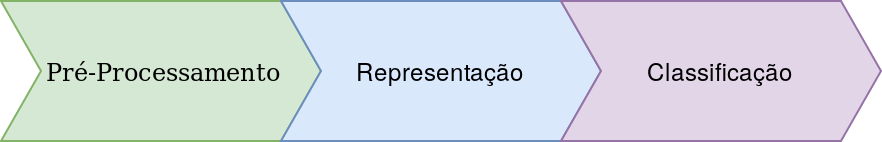
\includegraphics[scale=0.35]{images/nlp_diagram.png}
    \caption{Etapas de classificadores de Processamento de Linguagem Natural.}
    \label{fig:nlp_diagram}
    \end{center}
}
\end{center}
\end{figure}

\section{Pré-Processamentos}

A primeira etapa aplicada para a elaboração de modelos de NLP é o
pré-processamento.
Essa fase consiste na limpeza e preparação dos dados, visando a melhorar a
performance do classificador, seja retirando ruídos dos textos, reduzindo o
tamanho do vocabulário ou formatando o documento de maneira a facilitar a modelagem.

O volume do vocabulário adotado costuma ser limitado tanto pelos recursos
computacionais, quanto pelo requisito mínimo de estatística das palavras na base
de dados.
Portanto, técnicas de pré-processamento que reduzam o tamanho total do
vocabulário têm um importante papel na garantia de um bom funcionamento dos
classificadores.

Como a maior parte dos modelos de NLP trabalham a nível de palavra, é necessário
separar o documento em frases, com algoritmos como o Punkt~\cite{kiss06}, e,
posteriormente, em palavras.
Esse processo, chamado \textit{tokenização}, precisa ser robustos a abreviações,
números e outras características específicas do idioma ao qual será aplicado,
como a contração de palavras em português.
Se tratando de redes sociais, também é relevante tratar os links, as
\textit{hashtags} e as menções a usuários.

Algoritmos de correção ortográfica~\cite{damerau64}\cite{navarro01} podem ser
eficientes para aprimorar a qualidade dos textos, principalmente se tratando de
mensagens provindas de meios de comunicação como as redes sociais.

Técnicas de stemização consistem na extração do radical das palavras, como o
obtido pelo algoritmo de Porter~\cite{porter80}.
Um exemplo é dado com a palavra ``montanha'', que possuí radical ``mont'', o
mesmo obtido pela palavra ``monte''.
Por outro lado, o processos de lematização tem finalidade parecida, porém
transforma a palavra em sua forma base, isto é, forma como ela aparece no
dicionario, podendo então diferenciar palavras com o mesmo radical, como
``banco'' e ``bancários''.
Ambas as técnicas visam a tornar as etapas posteriores menos sensíveis a flexões
gramaticais, além de colaborar na redução do vocabulário.

Uma das principais etapas do pré-processamento é a remoção das
\textit{stopwords}, conjunto de palavras que contêm informação pouco discriminante
para uma dada aplicação~\cite{lo05}.
Geralmente, elas são compostas pelas palavras mais comuns da língua,
principalmente artigos e preposições.
O objetivo da remoção das \textit{stopwords} é diminuir ruídos dos dados
textuais, assim simplificando a etapa de modelagem.
\citet{saif14} fizeram um estudo comparando diversos métodos de seleção de
\textit{stopwords} e o impacto das mesmas na classificação de sentimento de
\textit{tweets}.
A identificação de classe gramatical, em inglês \textit{part-of-speech}, além de
ser tipicamente utilizada como entrada de modelos de NLP, também pode ser útil
para selecionar \textit{stopwords}.

\section{Representações}

Uma vez que os tratamentos iniciais dos textos são feitos, chega-se à etapa de
preparação desses dados para serem processados pelo modelo.
Para isso, os documentos são transformados de sequências de palavras em vetores
ou matrizes.
Há diversas técnicas desenvolvidas com essa finalidade, que podem ser divididas
em representações esparsas e densas.
As representações esparsas são as mais simples de serem aplicadas dado que, em
geral, não dependem do treinamento de nenhum modelo.
Entretanto, elas resultam em vetores ou matrizes de dimensão na ordem de, pelo
menos, o tamanho do vocabulário escolhido.
Como os vocabulários costumam ser muito extensos (centenas de milhares de palavras em
alguns casos), o tamanho e a esparsidade da representação obtida podem dificultar
o treinamento dos classificadores.
Para contornar essa dificuldade foram criados algoritmos de representações
densas.
Por transformarem os documentos em vetores ou matrizes de baixa dimensão, estes
algoritmos foram os responsáveis pela viabilidade de utilização de técnicas de
\textit{Deep Learning} aplicadas ao processamento de linguagem natural.
Nessa seção, descreveremos algumas das principais técnicas de representação de
texto.

\subsection{Codificação One-Hot}

A codificação \textit{One-Hot} representa cada palavra de maneira maximamente
esparsa.
Para tal, é definido um espaço vetorial em que cada palavra do vocabulário
utilizado é equivalente a uma dimensão do espaço.
Portanto, um documento pode ser transcrito dessa forma em uma sequência de
vetores, ou matriz, em que cada palavra é um vetor com valor unitário na
dimensão da própria palavra e zero nas outras, como mostra a
Figura~\ref{fig:onehot}.

\begin{figure}[h]
\begin{center} {
    \begin{center}
    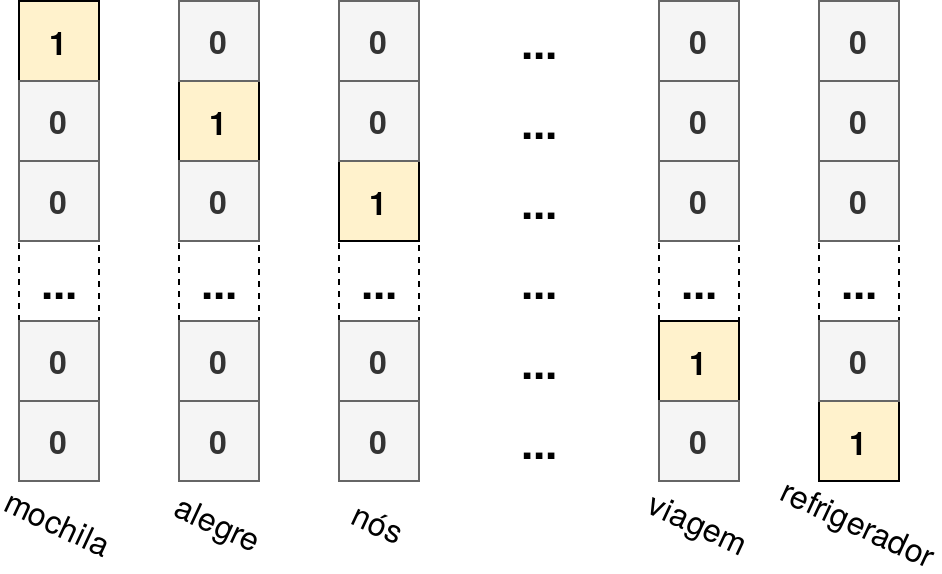
\includegraphics[scale=0.30]{images/onehot.png}
    \caption{Vetores \textit{One-Hot} de palavras de um dicionário.
             A dimensionalidade do vetor é igual ao tamanho do dicionário.}
    \label{fig:onehot}
    \end{center}
}
\end{center}
\end{figure}

Frequentemente encontramos nas línguas palavras compostas ou expressões.
Essas informações são perdidas na codificação \textit{One-Hot}.
Uma forma de se atenuar esse problema são com os chamados \textit{N-gramas}.
A ideia do \textit{N-grama} é formar tokens de 2, 3, ou \textit{n} palavras,
resultando em uma dimensionalidade equivalente à quantidade de
\textit{N-grama} do corpus formador do dicionário.
Entretanto, o aumento no número de palavras por token também gera um aumento
significativo do número de dimensões, dificultando o treinamento do
classificador.

\subsection{Bag-of-Words}

A codificação \textit{Bag-of-Words} é uma alternativa à representação de
mensagens como matrizes compostas de vetores \textit{One-Hot} de suas palavras.
Esta é feita pela soma desses mesmos vetores~\cite{manning10}.
Portanto, a representação final é dada por um único vetor, de tamanho
correspondente ao do vocabulário utilizado.
Esta técnica também tem a vantagem de transformar documentos de tamanho variados
em vetores de dimensões fixas, fator que precisa ser contornado em codificações
baseadas em palavras.

\begin{figure}[h]
\begin{center} {
    \begin{center}
    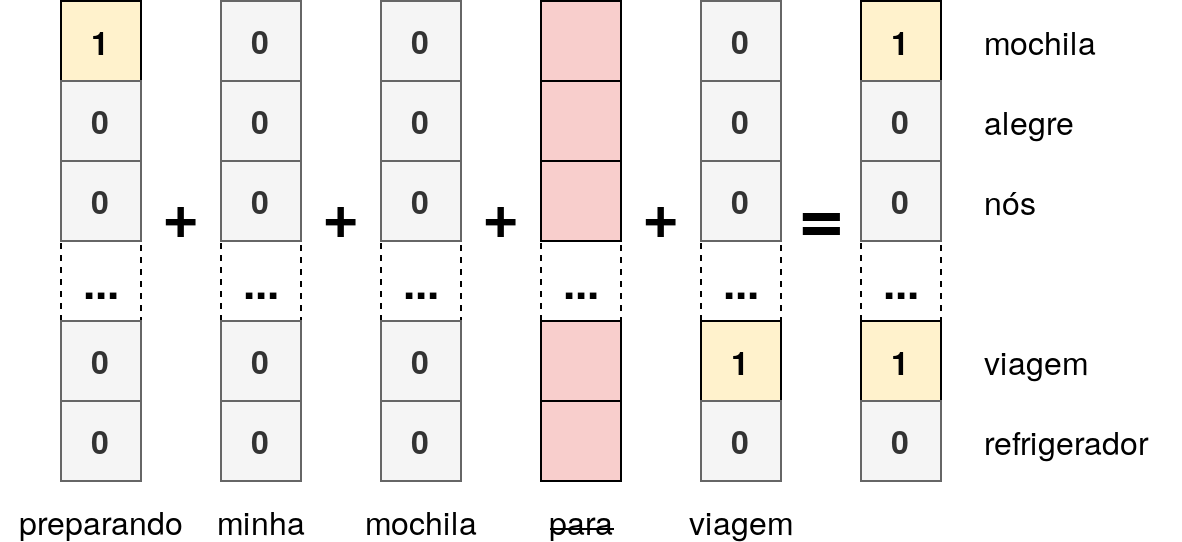
\includegraphics[scale=0.30]{images/bag_of_words.png}
    \caption{Processo de representação por \textit{Bag-of-Words} da frase
             ``Preparando minha mochila para viagem.''.
             A palavra ``para'' é removida durante o pré-processamento por
             ser uma \textit{stopword}.}
    \label{fig:bag_of_words}
    \end{center}
}
\end{center}
\end{figure}

Entretanto, a distribuição de palavras em um corpus, em geral, segue a lei de
Zipf~\cite{powers98}, ou seja, sua frequência segue uma distribuição em lei de
potência.
Sendo assim, mesmo retirando \textit{stopwords}, as palavras mais comuns do
vocabulário ainda dominarão os documentos e esse comportamento pode ser
prejudicial para o treinamento dos modelos que serão menos expostos a palavras
incomuns.

% TODO: exemplo zipf grafico ou equacao

Para atenuar tal problema, pode-se aplicar o \textit{term frequence-inverse
document frequence} (TF-IDF)~\cite{salton88}.
Nesse caso, a representação segue a mesma estrutura proposta pela codificação
\textit{bag-of-words}.
Entretanto, cada palavra é ponderada por um multiplicador inversamente
proporcional a sua frequência nos documentos.

% TODO: equação tf-idf

\textit{Bag-of-words} e TF-IDF são métodos de representação muito presentes na
literatura pela sua simplicidade de implementação e pelos benefícios
anteriormente descritos, em especial em conjunto com modelos como a
SVM (Seção~\ref{sec:svm}), que apresenta menos dificuldades de ser treinada em
dados esparsos.
No entanto, um componente fundamental da linguagem é perdido durante processo: o
contexto em que cada palavra se insere.
Pela representação agrupar todos os tokens em um único vetor, a ordem das
palavras no documento é perdida, o que em muitos casos pode corresponder à
inviabilidade de uma classificação precisa do mesmo.

% TODO: talvez mostrar exemplo em que a ordem faria diferença

As técnicas de representações densas que serão apresentadas a seguir, além de
resolverem o obstáculo da dimensionalidade dos dados, também viabilizam a
classificação por modelos que levem em conta o contexto de cada palavra.

\subsection{Word2Vec} \label{sec:w2v}

\textit{Word2Vec}~\cite{mikolov13} foi uma das primeiras técnicas de
representação densa de palavras amplamente adota pela indústria e pela academia.
Representações densas são aquelas em que cada palavra é transformada em um vetor
de números reais de baixa dimensionalidade, tipicamente dezenas ou poucas
centenas de dimensões.
\citet{mikolov13} mostraram que essa representação é capaz de capturar parte dos
sentidos semânticos e sintáticos das palavras, aproximando as que são sinônimas
ou exerçam a mesma função gramatical, atenuando assim o problema da disparidade
de frequência das palavras.

Esta técnica é um modelo constituído de uma rede neural de uma camada escondida.
Para o treinamento do mesmo, são feitas janelas de um número arbitrário de
palavras que servirão como entrada do modelo.
Dessas janelas, há duas variações: o \textit{continuous bag-of-words}, em que
o modelo é treinado para prever a palavra central da janela de entrada a partir
das outras palavras da janela, e o \textit{skipgram}, que a partir da palavra
central é treinado para prever o seu contexto.
A Figura~\ref{fig:w2v} ilustra a diferença entre esses métodos.
As entradas e saídas do modelo são representadas pela codificação
\textit{one-hot} dos termos.
A quantidade de neurônios escolhida para a camada escondida da rede resultará na
dimensionalidade da representação das palavras.
Estas, por sua vez, serão os pesos da camada de entrada do modelo treinado.

\begin{figure}%
    \centering
    \subfloat[Continuos Bag-of-Word]{{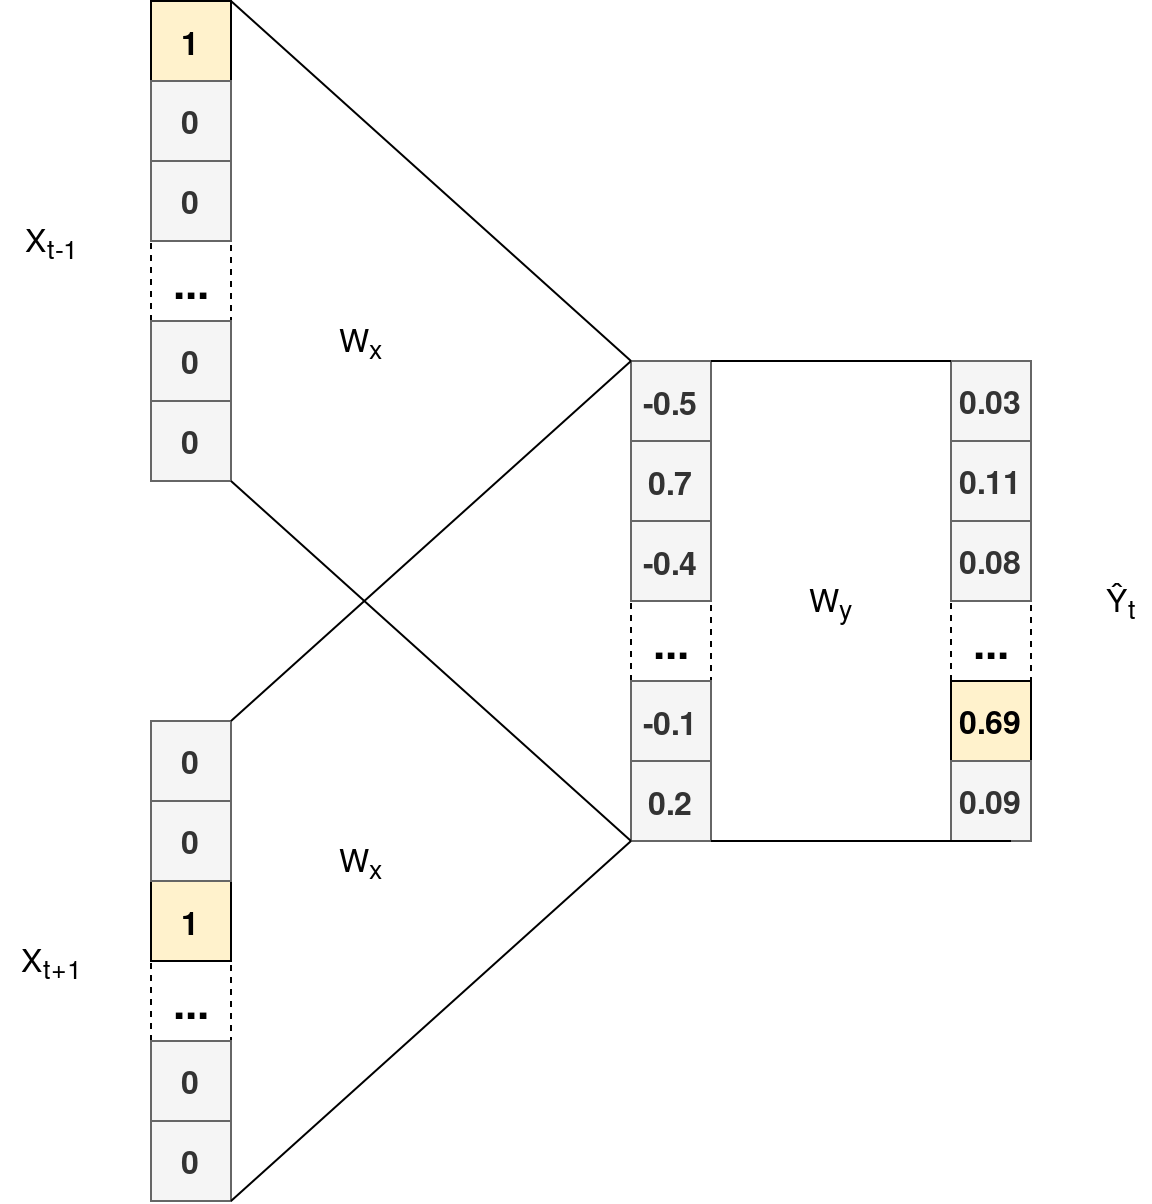
\includegraphics[scale=0.24]{images/word2vec_cbow.png}}}%
    \qquad
    \subfloat[Skipgram]{{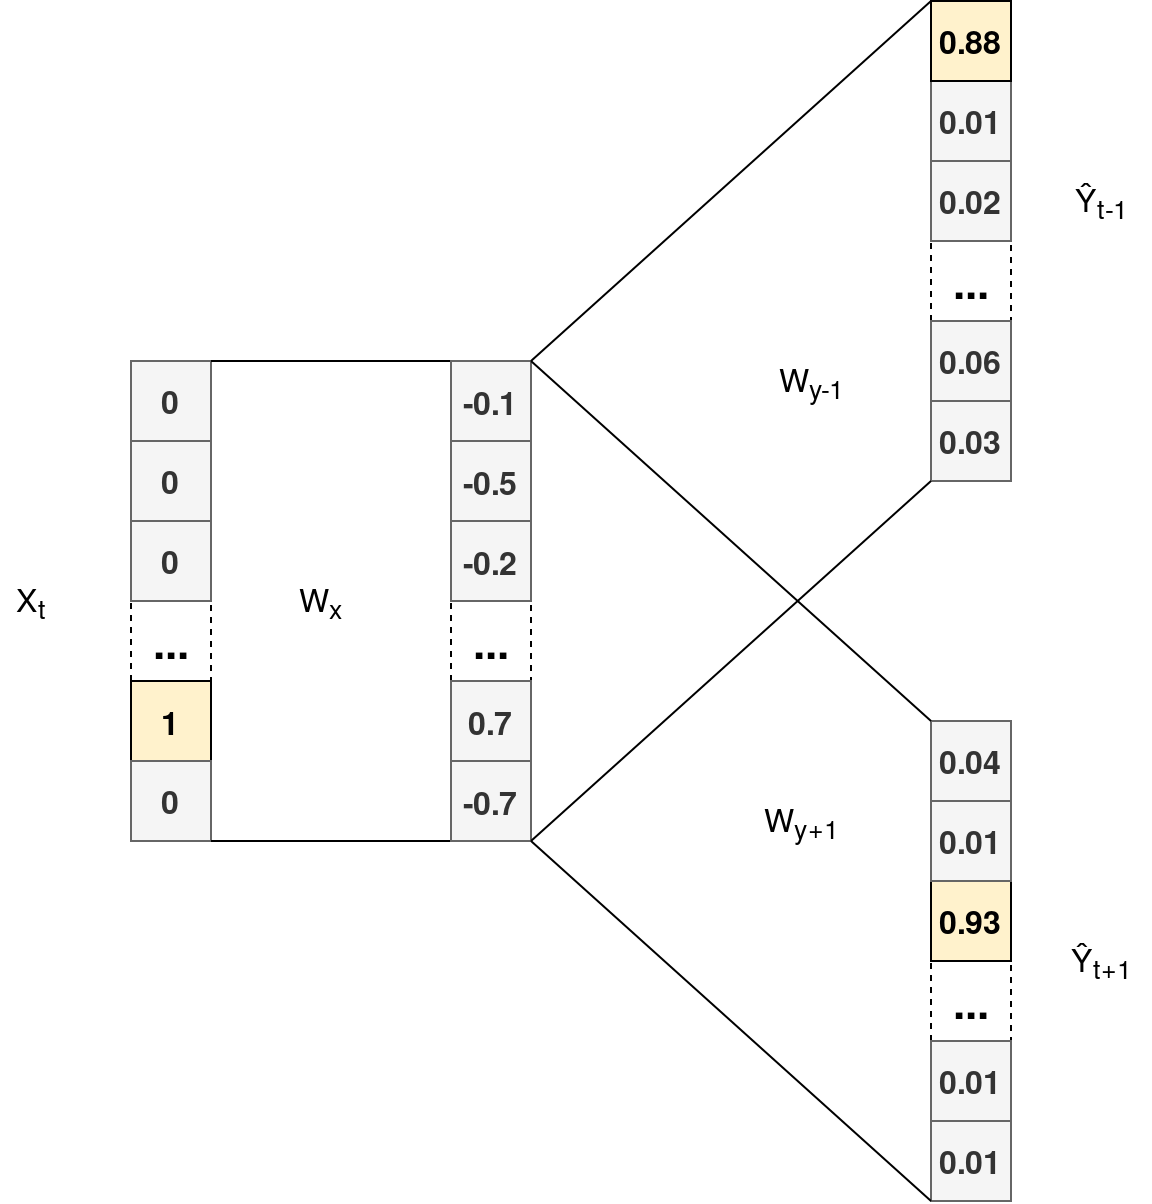
\includegraphics[scale=0.25]{images/word2vec_skip.png}}}%
    \caption{Esquemas de treinamento do Word2Vec. Exemplo composto por janela de
             contexto de 3 palavras. A matriz $X_t$ representa a palavra da
             janela na posição $t$ e $\hat{Y}_t$ a predição do modelo para a
             mesma. $W$, por sua vez, representa o conjunto de pesos treináveis.
             A representação resultante de uma palavra é dada pelo seu referente
             vetor na matriz de pesos de entrada $W_x$.}%
    \label{fig:w2v}%
\end{figure}

Apesar de o \textit{Word2Vec} ser um modelo que precisa ser treinando, esse
treinamento é não-supervisionado, dado que tanto as entradas quanto as saídas do
modelo são obtidas diretamente dos documentos, sem anotações de classes.
Desta forma, foi possível aplicar o algoritmo a grandes bases de dados
mineiradas da internet.
Esse tamanho volume de dados de treinamento foi essencial para que bons resultados
demostrados por \citet{mikolov13} fossem alcançados.

Por ser a primeira representação densa de sucesso, o \textit{Word2Vec} foi
essencial para a aplicação de classificadores também baseados em redes neurais,
como os de \textit{Deep Learning}, que obtiveram grande êxito em diversas
tarefas de processamento de linguagem natural.
Outras técnicas de representação densas semelhantes e também amplamente adotadas
na indústria foram desenvolvidas neste mesmo período de tempo, como o
GloVe~\cite{pennington14} e o FastText~\cite{bojanowski17}.

% TODO abrir matematica do W2V

\subsection{Representações por Redes Neurais Recorrentes}
\label{representation:rnn}

O sucesso do \textit{Word2Vec}, baseado em redes neurais \textit{feed forward},
inspirou a experimentação de outros tipos de redes neurais.
Dentre elas, redes neurais recorrentes e suas variações obtiveram bons resultados
na representação de palavras.
Nesta seção, serão descritas as variações deste algoritmos.

A estrutura chamada \textit{Enconder-Decoder}, desenvolvida por \citet{cho14},
se tornou a base das principais representações por redes recorrentes.
Ela consiste em uma rede neural recorrente divida em duas etapas: a codificação,
na qual uma sequência de tamanho variável é representada em um
vetor de contexto; e a decodificação, em que esse mesmo vetor é utilizado para
obter uma outra sequência de tamanho variável.
O \textit{Encoder-Decoder} é um modelo de aprendizado de sequências de tamanho
variável a partir de outra sequência de tamanho variável como entrada, não
necessariamente com os mesmos tamanhos.
Isso é reflexo do problema inicial que o mesmo foi desenvolvido para atacar: a
tradução de textos.

\begin{figure}
\begin{center} {
    \begin{center}
    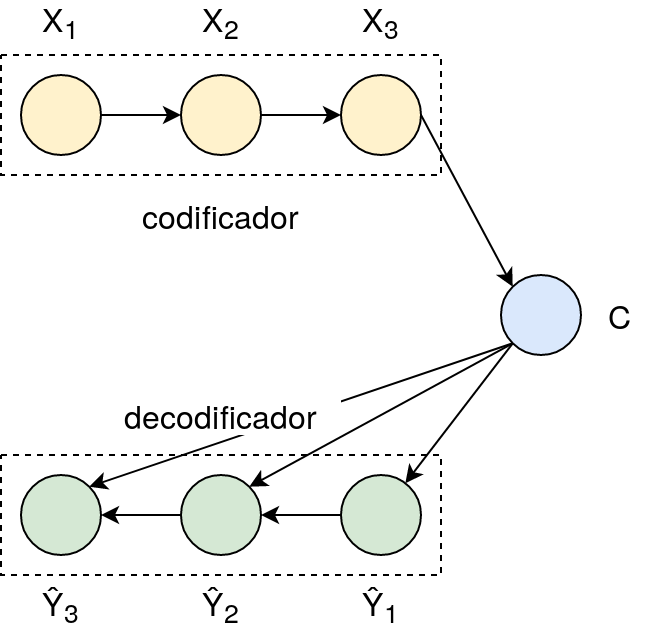
\includegraphics[scale=0.30]{images/encoder_decoder.png}
    \caption{Arquitetura Encoder-Decoder, constituída por duas camadas de redes
             recorrentes: a de codificação e a de decodificação, ligadas por um
             conjunto de pesos $C$, que captura todo o contexto provindo da
             camada de codificação.}
    \label{fig:encoder_decoder}
    \end{center}
}
\end{center}
\end{figure}

Toda essa estrutura é treinada conjuntamente e pode ser utilizada para gerar
sequências de saída a partir de entradas, ou para avaliar um par de entrada e
saída a partir da probabilidade $p_{\mathbf{\theta}}(\mathbf{y} \mid \mathbf{x})$.
Esta última sendo aprendida pelo treinamento, no qual $\mathbf{x}$ e $\mathbf{y}$
representam respectivamente as sequências de entrada e saída e $\mathbf{\theta}$
o conjunto de pesos do modelo treinado.

A etapa de codificação desse modelo pode ser vista como um resumo da sequência
de entrada em um vetor de tamanho fixo.
Assim sendo, o mesmo pode ser utilizado para representações de documentos ou
frases, ou até mesmo de palavras, caso aplicada uma sequência de tamanho unitário.
\citet{cho14} demostram brevemente em seu trabalho que a codificação é capaz de
capturar significados semânticos e sintáticos das palavras, assim como o Word2Vec.

\subsubsection{ELMo}
% Deep contextualized word representations

ELMo~\cite{peters18}, sigla para \textit{Embeddings from Language Models}, em
português Representações para Modelos Linguísticos, é um modelo capaz de obter
representação de palavras, e se diferencia de modelos de representação de
palavras como o Word2Vec por levar em consideração o contexto da palavra para
obter sua representação, tanto durante o treinamento, quanto durante a
inferência.
Isto é, uma palavra que possua múltiplos sentidos terá representações diferentes
dependendo da frase em que está inserida.
A ideia de utilizar o contexto da palavra para selecionar sua representação
durante a inferência foi inspirado pelos trabalhos de \citet{peters17} e
\citet{mccann17}.
O modelo é composto de uma rede LSTM~\cite{hochreiter97} bidirecional e com
múltiplas camada, treinada de maneira não supervisionada a partir do objetivo de
prever a palavra seguinte.

% TODO: diagrama ELMo para esclarecer 1 paragrafo (ver http://jalammar.github.io/illustrated-bert/)

Estudos anteriores mostram que em modelos de redes recorrentes multicamadas,
a melhor camada escolhida para representação das palavras depende da finalidade
em que se deseja aplicá-la
~\cite{hashimoto16}~\cite{sogaard16}~\cite{belinkov17}~\cite{melamud16} e que,
em geral, camadas inferiores codificam melhor a informação sintática e camadas
superiores a informação semântica.
A proposta de ELMo é, para cada tarefa, treinar uma combinação linear das
representações obtidas por cada camada da rede.

\citet{peters18} ressaltam que ELMo foi capaz de obter resultados significativamente
melhores que as técnicas do estado da arte até então, considerando diversas tarefas
do processamento de linguagem natural.
Além de capturar informação sintática e semântica, ELMo se mostrou capaz de
desambiguar o contexto de palavras, problema até então não resolvido pelos
principais algoritmos de representação.

\subsection{BERT}
% bert - 2018 - BERT: Pre-training of Deep Bidirectional Transformers for Language Understanding

Outra técnica de representação bastante utilizada atualmente para representação
de palavras é a BERT~\cite{devlin18}, \textit{Bidirectional Transformers}.
No entanto, antes de explicá-la, será apresentada abaixo a arquitetura
Transformers, em que a mesma se baseia.

\subsubsection{Transformers}
% transformers - 2017 - Attention is all you need (boa explicacao dos conceitos)

Um dos principais problemas de redes neurais recorrentes é o ``esquecimento''.
O esquecimento é observado quando se perde influência das primeiras palavras de
uma longa sequência ao se tentar prever a palavra no final da mesma.
Essa situação decorrente das sucessivas funções de ativação dos neurônios entre
as palavras do começo e do final do documento.
Mesmo com o algoritmo LSTM~\cite{hochreiter97}, \textit{Long-Short Term Memory},
que visa a atenuar esse efeito criando um peso adicional, chamado de portão (que
controla o quanto os pesos de contexto são atualizados entre cada iteração de
palavras de uma sequência), o esquecimento continua sendo um fator limitante.

O mecanismo de atenção desenvolvido por \citet{bahdanau14} também tem como
objetivo diminuir o efeito do esquecimento.
Este consiste em um conjunto de pesos adicionais que, multiplicados pelos pesos
de estados das iterações anteriores, formam os pesos de estado da iteração
corrente, como também descrito em mais detalhes por \citet{luong15}.
A atenção se tornou uma das principais adições feitas a redes recorrentes
aplicadas a processamento de linguagem natural.

% TODO: figura mostrando atencao (luong15 tem figura)

Inspirado nesse mecanismo, \citet{vaswani17} propuseram a arquitetura
Transformer para tradução de textos.
Essa arquitetura consiste em um sistema de \textit{Encoder-Decoder}, desta vez
composto por redes neurais \textit{feed forward} multi camadas.
Nelas a dependência temporal entre as palavras de um documento é atacada apenas
pelo sistema de \textit{self-attention}, ou de atenção própria.

Enquanto o mecanismo de atenção se dá por um único conjunto de pesos, a
\textit{self-attention} é dividida em 3: os pesos de busca, de resposta e de
valor.
Cada palavra do vocabulário terá um de cada vetor citado acima associado a ela.
Para cada palavra do documento, será feito um produto interno do seu vetor de
busca e os vetores de resposta das outras palavras da sentença, resultando em um
valor único de atenção entre cada par possível de palavras de uma sentença.
Após calcular esse valor, será realizada uma operação de Softmax para que a norma
do vetor de atenção seja unitária.
Posteriormente, se multiplica o vetor resultante pelo vetor de valor da palavra
de resposta.
Essa operação tem a finalidade de diminuir a importância de palavras sem
potencial discriminatório, como as \textit{stopwords}.
Assim são calculadas as entradas da camada \textit{feed forward} do algoritmo.

A etapa de codificação do Transformer é composta por uma cascata de unidades
formadas por uma camada de \textit{self-attention} seguida de uma camada de
rede \textit{feed forward}.
A Figura~\ref{fig:transformer_layer} ilustra uma camada da arquitetura descrita.
Diferentemente das redes recorrentes, o Transformer requer um tamanho fixo de
entrada, sendo um parâmetro a ser definido dependendo da base de treinamento
escolhida.
Apesar de as redes \textit{feed forward} não possuírem um conceito de sequência,
como as redes recorrentes, essa arquitetura provou ser eficiente em tarefas de
processamento de linguagem natural, ao passo que possui treinamento
significativamente menos custoso que a redes recorrentes~\cite{vaswani17}.

\begin{figure}
\begin{center} {
    \begin{center}
    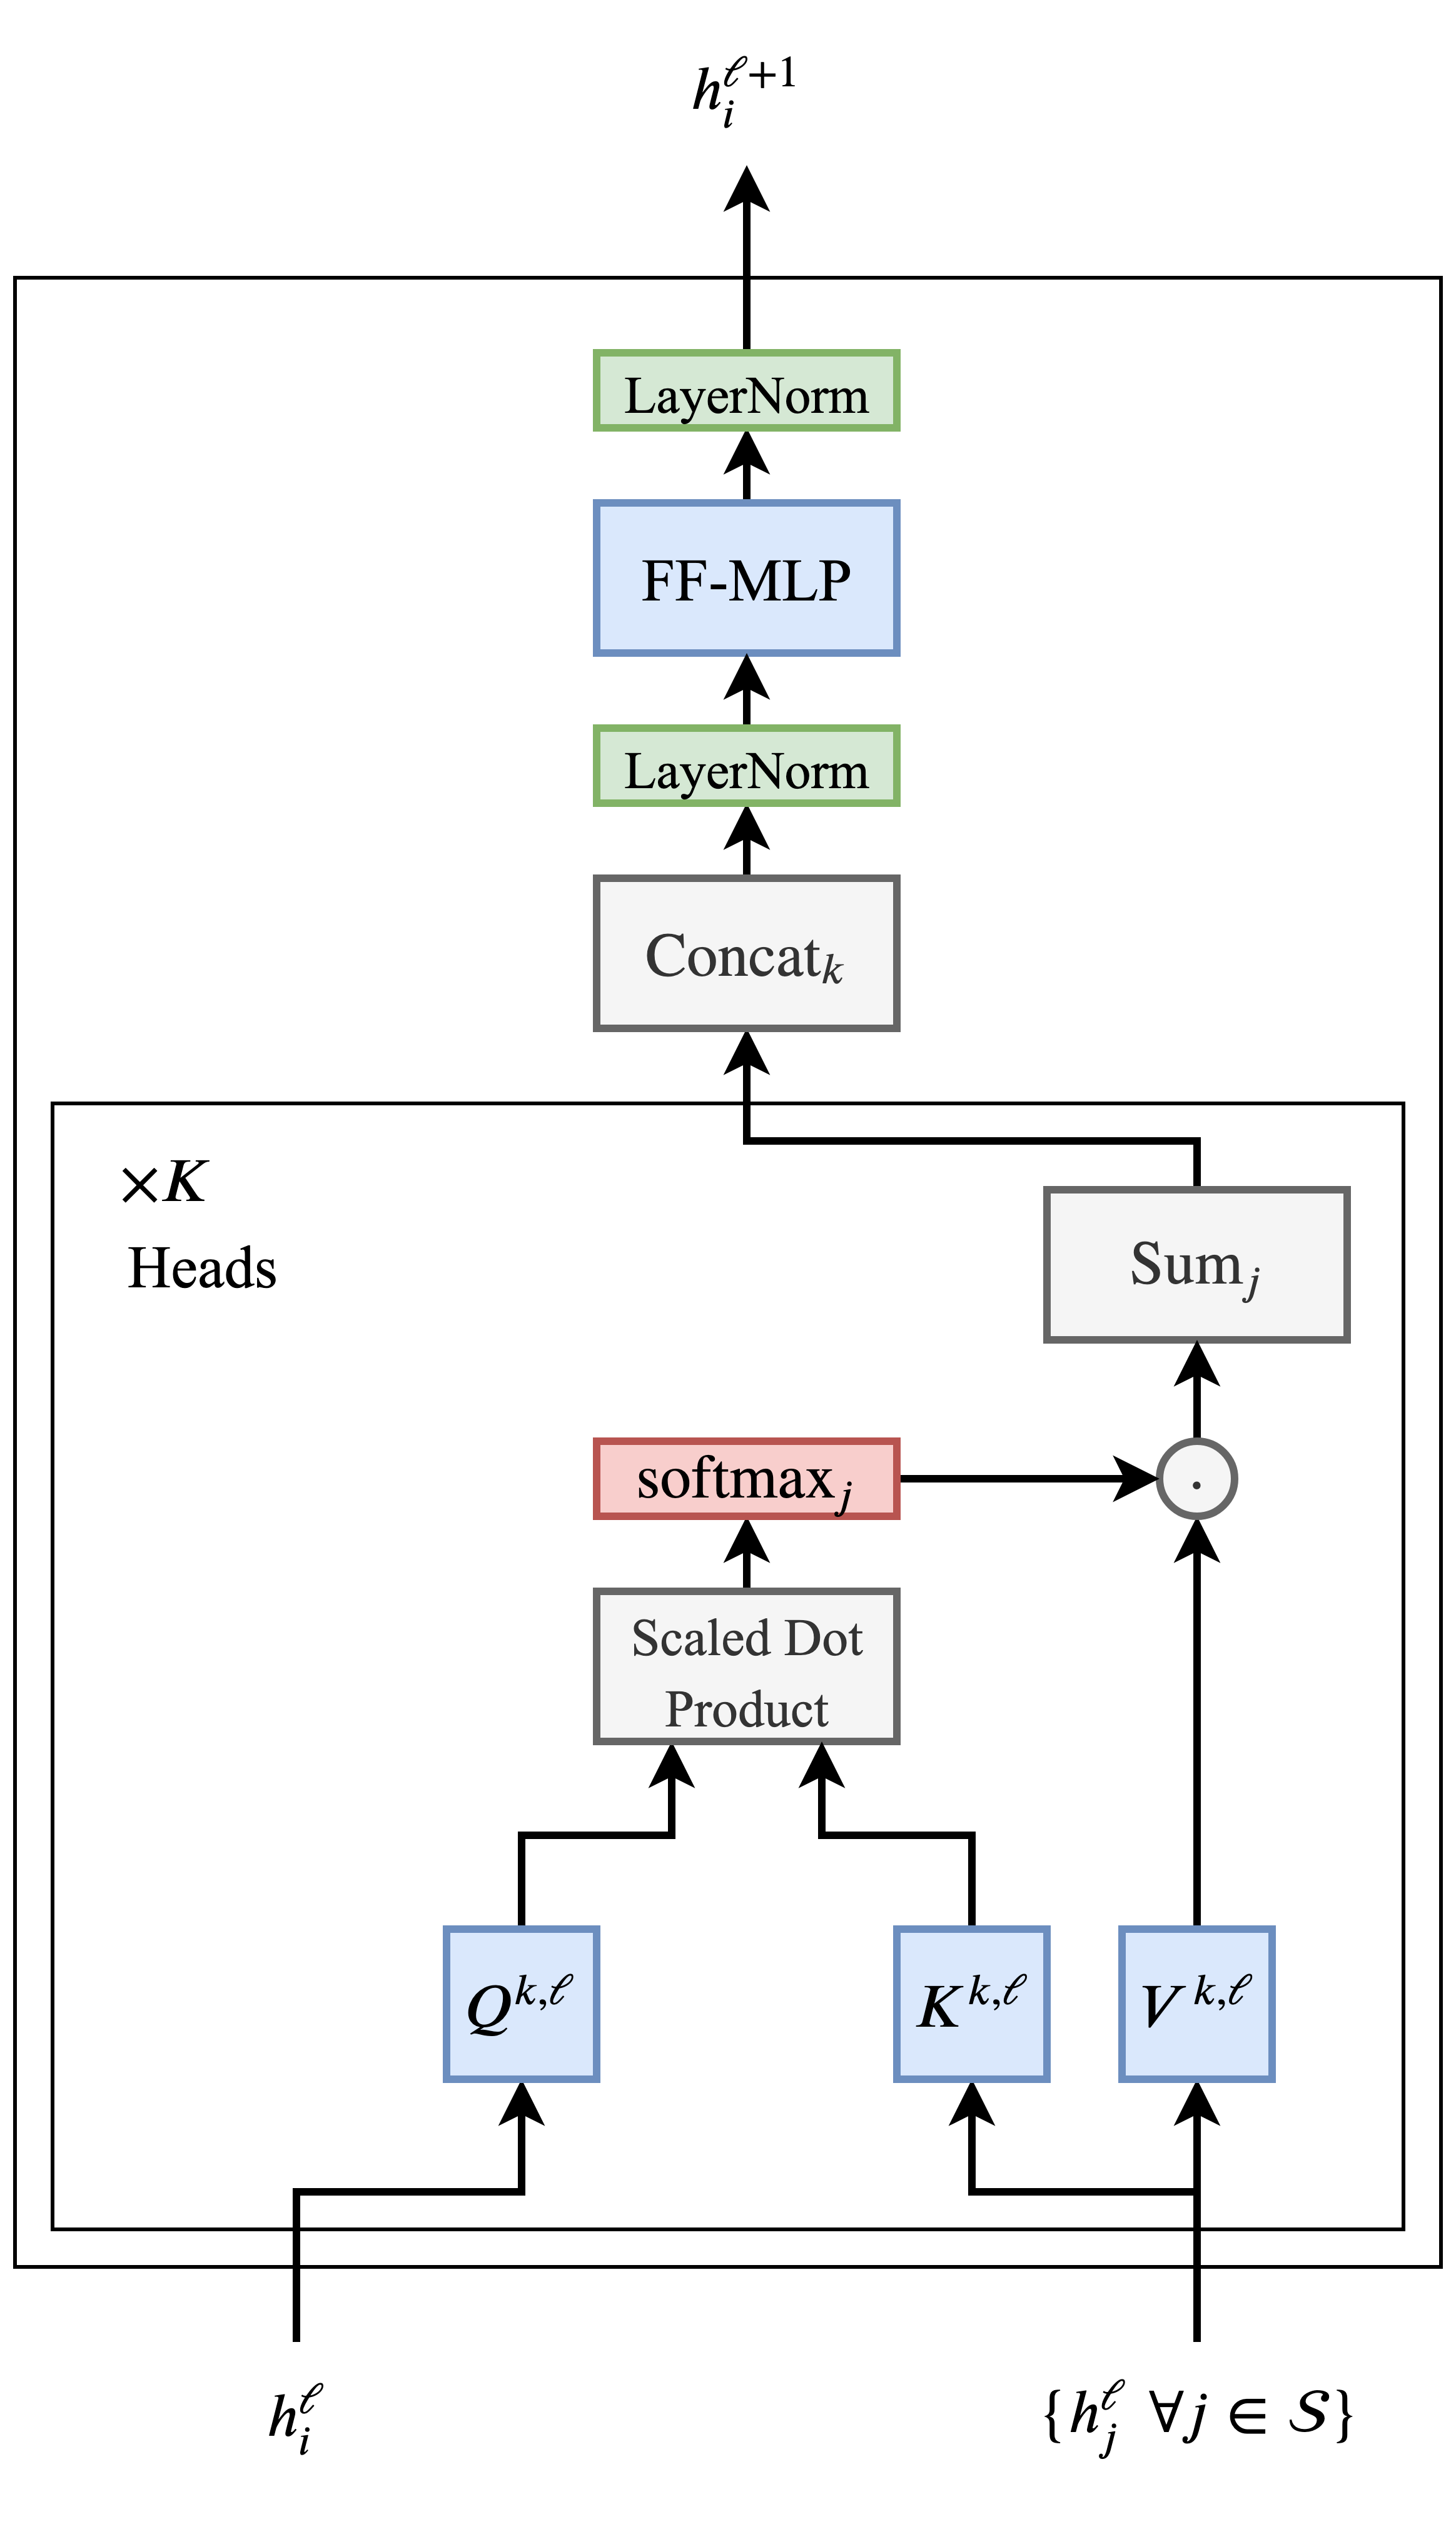
\includegraphics[scale=0.8]{images/transformer_layer.png}
    \caption{Diagrama da camada $\ell$ do Transformer com K cabeças de
             \textit{self-attention} para uma palavra de índice $i$, dada a
             sentença $S$.
             As matrizes $Q^{k,\ell}$, $K^{k,\ell}$ e $V^{k,\ell}$ representam
             respectivamente os pesos de atenção de busca, resposta e valor.}
    \small Figura retirada de~\cite{joshi20}.
    \label{fig:transformer_layer}
    \end{center}
}
\end{center}
\end{figure}

\subsubsection{Arquitetura BERT}

O sucesso do Transformer em traduções inspirou sua aplicação em outras tarefas.
\citet{radford18} propuseram utilizar apenas a camada de decodificação do
Transformer, junto com uma adaptação da sequência de entrada, para adequar a
tarefa a ser realizada.
O modelo é pré-treinado com uma quantidade massiva de dados na predição da
palavra seguinte e posteriormente é feito um ajuste fino com uma base de dados
da tarefa desejada.
Essa nova arquitetura foi capaz de propagar os ganhos de performance do Transformer
para toda a gama de tarefas de NLP.

Entretanto, tanto o Transformer original quanto o de \citet{radford18} são
modelos unidirecionais, prevendo a palavra, ou sentença à direita, a partir do
contexto à esquerda.
\citet{devlin18} defendem que, por serem unidirecionais, os modelos possuem
capacidade limitada, principalmente em tarefas que utilizam a sentença
inteira, sendo a análise de sentimento um exemplo.
Proporam, então, um modelo bidirecional praticamente idêntico ao Transformer de
\citet{radford18} sendo sua única modificação ter o mecanismo de atenção
considerando bidirecionalmente o contexto.

Além de representar palavras, o BERT pode ser usado diretamente como
classificador, assim como o ELMo.
\citet{devlin18} mostram as diferenças entre as camadas do modelo quando
utilizado como representação.
Assim como nas arquiteturas apresentadas anteriormente, as diferentes camadas
possuem aprendizado de características distintas da língua.

\section{Classificadores}

Nessa seção serão abordadas as diferentes estratégias para classificação de
sentimento.
As etapas descritas anteriormente lidam com a preparação dos documentos para
a realização da classificação.
Mesmo com complexidade dos métodos apresentados, os classificadores podem ser
tão simples quanto contadores de palavras positivas e negativas.
Podemos dividi-los em algoritmos baseados em dicionário e algoritmos de
aprendizado de máquina~\cite{taboada11}, estando suas respectivas
características descritas abaixo.

\subsection{Algoritmos Baseados em Dicionários} \label{sec:dictionary}

Uma das técnicas mais simples para a classificação de sentimento é feita a partir
da elaboração de um dicionário composto por palavras que tenham conotação
positiva ou negativa.
A formação de um dicionário de sentimento pode ser feita de forma
manual~\cite{stone66}~\cite{tong01} ou de forma automática.
Dentre as maneiras automáticas, temos a aplicada por \citet{hu04}, que é feita a
partir de um conjunto inicial de palavras anotadas e de um dicionário de
sinônimos e antônimos, tal qual o WordNet~\cite{miller90}.
Um exemplo é selecionar as palavras semente ``bom'' e ``ruim'' e montar uma base de
palavras recursivamente a partir dos seus sinônimos e antônimos.
Formas similares de identificação de palavras com sentimento baseada em
dicionários e palavras semente foram desenvolvidas por \citet{blair08},
\citet{rao09}, \citet{hassan10}, entre outros.

Existindo um dicionário, a classificação de polaridade de um documento é dada
a partir de alguma função dos sentimentos das palavras que o compõem.
É comum a inclusão de algumas características sintáticas como a identificação de
adjetivos intensificadores e de identificação de negação, para ponderar a pontuação
de sentimento de uma palavra ou expressão~\cite{taboada11}.
A função de classificação pode ser tão simples quanto uma média do sentimento
das palavras ou, por exemplo, um calculo de proximidade entre o conjunto de
palavras do documento e as palavras ``excelente'' e ``ruim'', representando as
classes positivas e negativas, como propõe \citet{turney02}.

% pang and lee 2008 4.5.1
% Lexicon-Based Methods for Sentiment Analysis
% Liu 2012 sentiment analysis
% Mining and Summarizing Customer Reviews tem boas referencias no 2.2

\subsection{Modelos de Aprendizado de Máquina Lineares}

Naturalmente, as primeiras aplicações de aprendizado de máquina em análise de
sentimento fizeram uso de modelos simples, como os lineares.
\citet{pang02} fizeram um dos primeiros estudos comparativos entre esses
métodos.
A seguir, serão descritos os dois principais modelos lineares utilizados em
processamento de linguagem natural: Naïve Bayes e Máquina de Vetor de Suporte.

\subsubsection{Naïve Bayes}

O classificador de Naïve Bayes se baseia no teorema de Bayes
(Equação~\ref{eq:bayes}) e na premissa de independência entre as dimensões da
representação dos dados.
Quando representamos um documento textual com, por exemplo, \textit{bag-of-words},
a premissa de independência significa assumir que existe independência entre as
palavras do documento.
Apesar de não existir independência entre palavras na linguagem, tal modelo foi
amplamente aplicado a tarefas de processamento de texto, devido a sua performance
e simplicidade.

\begin{equation} \label{eq:bayes}
    P(A\mid B) = \frac{P(A) P(B \mid A)}{P(B)}
\end{equation}

\citet{schutze08} descreveram a formulação matemática desse modelo, como será
demostrado.
Será denominado $\mathbf{X}$ o corpus de treinamento e $\mathbf{x}$ um documento
desse corpus.
As classes a que os documentos pertencem, como positiva e negativa, são chamadas de
$c_k$, na qual $\mathbf{c}$ é o conjunto de classes.
Portanto, substituindo as variáveis da equação~\ref{eq:bayes} tem-se que a
probabilidade de um documento pertencer a uma determinada classe é dada por:

\begin{equation}
    p(c_k \mid \mathbf{x}) = \frac{p(c_k) \ p(\mathbf{x} \mid c_k)}{p(\mathbf{x})}
\end{equation}

Como se assume independência entre as variáveis, tem-se que:

\begin{equation}
    p(x_i \mid x_{i+1}, \dots ,x_{n}, c_k ) = p(x_i \mid c_k)
\end{equation}

Logo, pode-se substituir $p(\mathbf{x} \mid c_k)$ pelo produtório de
$p(x_i \mid c_k)$:

\begin{equation}
    p(c_k \mid \mathbf{x}) = \frac{p(c_k) \prod_{i=1}^n p(x_i \mid c_k)}{p(\mathbf{x})}
\end{equation}

A probabilidade $p(\mathbf{x})$ será constante, logo não influenciará o
treinamento.
Assim tem-se que a relação entre a probabilidade de um documento
pertencer a classe é dada por:

\begin{equation}
    p(c_k \mid \mathbf{x}) \propto p(c_k) \prod_{i=1}^n p(x_i \mid c_k)
\end{equation}

Dessa forma, a tarefa da classificação, que é encontrar a classe de maior
probabilidade, é representada por:

\begin{equation}
    \hat{y} = \operatorname{max} p(c_k \mid \mathbf{x}) = \underset{k \in \{1, \dots, K\}}{\operatorname{max}} \ p(c_k) \displaystyle\prod_{i=1}^n p(x_i \mid c_k)
\end{equation}

A dependência entre a predição e o conjunto de treino, então, é dada por $p(c_k)$
e $p(\mathbf{x} \mid c_k)$.
Esses valores são obtidos por estimadores de máxima verossimilhança.
O parâmetro $p(c_k)$ é dado pela proporção de vezes em que a classe aparece no
conjunto de treino, tendo o conjunto de treino o tamanho $m$ de documentos:

\begin{equation}
    \hat{p}(c_k) = \frac{\sum_{i=1}^m [y_i = c_k]}{m}
\end{equation}

Por sua vez, $p(x_r \mid c_k)$ é estimado pela proporção entre uma determinada
característica $x_r$ e o total de características do subconjunto de dados
$\mathbf{X_{c_k}}$ pertencentes a classe $c_k$:

\begin{equation}
    \hat{p}(x_r \mid c_k) = \frac{\sum_{j=i}^{m'} \sum_{i=1}^n [x_{ji} = x_r]}{|\mathbf{X_{c_k}}|}
\end{equation}

O Naïve Bayes pode ser aplicado tanto a vetores inteiros da representação
\textit{bag-of-words} de frequência de palavras em um documento, quanto pelo seu
equivalente binário que assinala ou não a presença de uma determinada palavra.
Ao considerar a frequência de palavras, aplicamos o modelo multinomial, enquanto
ao utilizar a representação de forma binária temos o modelo de Bernoulli.
O modelo de Bernoulli é mais eficiente para documentos e vocabulários pequenos,
ao passo que o multimodal se sobressaí no caso oposto~\cite{schutze08}.

Apesar de a premissa de independência não ser verdadeira para a linguagem e não
ser um bom estimador de probabilidade das classes~\cite{schutze08}, Naïve Bayes se
mostra eficiente na classificação, em especial quando existe um conjunto de
características de semelhante importância.
Sua principal vantagem se dá pelo baixo custo computacional de treinamento, visto
que seus parâmetros são estimados apenas por contagens na base de dados.

\subsubsection{Máquina de Vetor de Suporte}
\label{sec:svm}

A Máquina de Vetor de Suporte, também chamada de SVM, é um algoritmo que busca
encontrar um vetor que melhor separe duas classes.
A diferença entre esse algoritmo e outros classificadores, como a regressão
linear, é que o SVM tem como objetivo obter o vetor que maximize a distância entre
as margens das classes.
A regressão linear, por sua vez, geralmente minimiza uma função custo baseada na
distância entre os dados e o centro de massa das classes.

\begin{figure}
\begin{center} {
    \begin{center}
    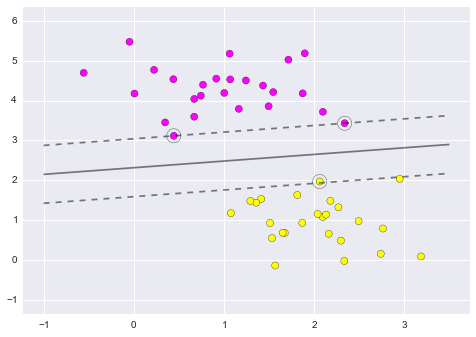
\includegraphics[scale=0.6]{images/svm.png}
    \caption{SVM classificando duas classes linearmente separáveis.}
    %\small Imagem com direitos cedidos para uso não comercial, retirada de~\cite{vanderplas15}
    \small Figura retirada de~\cite{vanderplas15}.
    \label{fig:svm}
    \end{center}
}
\end{center}
\end{figure}

Entretanto, por se basear na margem das classes, o SVM não é capaz de separar
classes que tenham sobreposição.
Como maneira de contornar esse problema, foi criada uma variável de relaxamento de
que controla o quanto de sobreposição é permitido entre as classes, como
explicam \citet{cortes95}.
Ainda assim, até então a Máquina de Vetor de Suporte fica limitada a problemas
lineares.
Apenas com o desenvolvimento do chamado \textit{kernel trick} é que o SVM pôde ser
aplicado à problemas não-lineares, ganhando assim alta adoção.
O \textit{kernel trick} consiste em realizar uma transformação na representação
dos dados de forma que os mesmos sejam linearmente separáveis após a
transformação.
Mapeamentos radiais e polinomiais são dois dos exemplos de \textit{kernel}
amplamente utilizados.

Uma das principais propriedades do SVM é que seu treinamento independe da
dimensionalidade das características dos dados, visto que seu aprendizado é feito
com base nas margens entre as classes.
Assim, uma vez que os dados sejam separados por uma margem, mesmo que tenham
alta dimensionalidade, o vetor de suporte de classificação pode ser encontrado.
A aplicação de SVM para classificadores de texto foi proposta por
\citet{joachims98}, visto que dados textuais representados por
\textit{bag-of-words} possuem 3 propriedades que se adéquam à classificação por
SVM:
\begin {enumerate*} [label=\itshape\alph*\upshape)]
    \item possuem alta dimensionalidade
    \item são esparsos
    \item tem poucas dimensões irrelevantes.
\end {enumerate*}
Apesar de \citet{joachims98} demostrar a efetividade do SVM para classificação
de texto utilizando \textit{kernels} não lineares, bons resultados são obtidos
mesmo sem a aplicação de \textit{kernel}, como mostram \citet{pang02}.

\subsection{Modelos de Aprendizado de Máquina Não-Lineares}

Classificadores lineares a partir de representação por \textit{bag-of-words} ou
TF-DF dos textos foram o estado da arte em tarefas de processamento natural
durante anos.
Entretanto, como visto anteriormente, ao aplicar técnicas como
\textit{bag-of-words}, abre-se mão do contexto em que cada palavra aparece no
documento.
Ta fator limita a performance da classificação.
Sem conseguir capturar o contexto, essas técnicas se distanciam de como
interpreta-se a língua.
Para diminuir essa lacuna, possibilitados pelo desenvolvimento de técnicas de
representações densas, passou-se utilizar classificadores não-lineares que
visam a adicionar alguma forma de contexto ao processo.

\subsubsection{Deep Learning}

Dentre os modelos não-lineares, os que mais se destacam em processamento de
linguagem natural são os de \textit{Deep Learning}, baseados em redes neurais.
Uma das principais características das redes neurais é serem algoritmos
capazes de aproximar qualquer função~\cite{hornik89}.
Com o desenvolvimento do método de treinamento por auto diferenciação, chamado
de \textit{backpropagation}, nos anos 80~\cite{werbos82} as redes neurais
foram amplamente adotadas.
Entretanto, dois principais fatores inviabilizaram o treinamento de redes
neurais de larga escala por muitos anos: o custo computacional do
\textit{backpropagation} e o efeito do \textit{vanishing gradient}~
\cite{hochreiter98}.
O \textit{vanishing gradient} é decorrente do efeito multiplicativo do
gradiente desde a camada de neurônios da saída até a camada de entrada.
O mesmo resulta em um treinamento menor da camada à medida em que ela está
mais distante da saída, estabelecendo assim uma dificuldade exponencial no
treinamento com relação ao número de camadas da rede.

Com o desenvolvimento tecnológico e a elaboração de uma técnica de treinamento
camada-a-camada, foi possível se sobrepor a esta barreira.
Nesse método, proposto por \citet{hinton06}, cada camada de neurônio
é treinada individualmente e os valores obtidos por esse treinamento são
utilizados como inicialização do treinamento da rede completa.
Após esse trabalho, começaram a testar redes neurais com um número cada vez
maior de camadas.
Denominou-se \textit{Deep Learning} o conjunto de modelos de redes neurais
profundas.

O salto de performance obtido pela aplicação de redes neurais
profundas~\cite{lecun15} em diversas áreas de conhecimento fez deste conjunto de
técnicas um objeto de estudo de muito interesse por pesquisadores e para indústria.
Parte de seu sucesso se atribuí ao fato de que cada adicional na rede neural
permite que a mesma obtenha uma representação mais complexa dos dados.
Considerando o processamento de linguagem, diferentes tipos de redes neurais
foram testados para tentar capturar a complexidade dessa informação,
com diferentes abordagens para adicionar o contexto em que cada palavra se
insere no processo de modelagem.
As seções abaixo descrevem os principais tipos de redes neurais aplicados a NLP.

% diferença principal de deep p tradicional é: contexto
% inspiração: http://dataskeptic.com/blog/episodes/2019/natural-language-processing

\subsubsection{Redes Neurais Convolucionais}

As redes convolucionais foram desenvolvidas prioritariamente para resolver
problemas como a classificação de imagens e o reconhecimento de fala.
Um fator comum que essas tarefas compartilham é a possível translação da
informação.
Na classificação de imagens, por exemplo, um determinado objeto pode estar em
diferentes posições ou ocupar tamanhos distintos em diferentes imagens.
Apesar de ser possível aplicar redes neurais MLP ao problema, esta precisaria
aprender os mesmos padrões de neurônios em diferentes posições~\cite{lecun95}.
Além disso, nesse tipo de problema existe uma característica da localidade da
informação.
Por exemplo, para reconhecimento de fala de uma palavra no final de uma frase,
a palavra imediatamente anterior é, em geral, mais importante que a primeira
palavra da mesma.
Ao se utilizar redes neurais MLP completamente conectadas entre camadas,
despreza-se essa propriedade, incorrendo em um maior custo computacional sem que
necessariamente se reflita em performance ou, pior, aumentando a chance de o
treinamento resultar em \textit{overfitting}.

A solução para a rede convolucional atacar o problema da correlação espacial da
informação é utilizar filtros espaciais.
Cada uma de suas camada é formada por um conjunto de filtros que são
compostos por neurônios.
A iteração de treinamento da rede consiste no deslocamento de cada filtro por
toda a dimensão da camada anterior.
Desta maneira, os padrões locais são capturados por um mesmo filtro
independente de onde os padrões apareçam nos dados de entrada.
O deslocamento dos filtros durante o treinamento funciona como um
compartilhamento de pesos, reduzindo a quantidade de parâmetros livres da rede
e, logo, sua probabilidade de \textit{overfitting}.

A interpretação de redes convolucionais aplicadas a processamento de texto não é
muito diferente de sua utilização com imagens.
Enquanto os filtros convolucionais exploram os padrões locais com filtros 2D de
poucos pixeis em imagens, no caso textual os filtros são unidimensionais e
percorrem a sequência de vetores de palavras com uma janela, capturando assim
parte do contexto em que cada palavra se insere.
Esse modelo já havia sido aplicado a documentos representados com
\textit{bag-of-words}, como demostrado por \citet{kalchbrenner14} e
\citet{yih14}.
Entretanto, apenas quando utilizado em conjunto com a representação
Word2Vec, como apresentou \citet{kim14}, esse algoritmo ganhou tração nas
tarefas de classificação de texto.
A disponibilidade de modelos Word2Vec pré-treinadas, somada à representação
densa que resulta em menor quantidade de parâmetros e menor probabilidade de
\textit{overfitting}, torna essa combinação acessível para treinamento mesmo em
casos de grandes bases de dados, dessa forma resultando em performance superior,
como mostra \citet{kim14}.

\subsubsection{Redes Neurais Recorrentes}

Outra forma de encapsular o contexto presente na linguagem é utilizando redes
neurais recorrentes.
Elas são, em geral, treinadas com o algoritmo
\textit{Backpropagation Through Time}~\cite{williams95} (BPTT).
Nesse algoritmo a rede recorrente se comporta como uma rede neural
\textit{feed-forward} na qual cada camada representa um passo temporal nos dados
de entrada.
No caso dos dados serem textuais cada passo pode ser uma palavra.
Portanto, ao aplicar esse algoritmo sobre o texto, o contexto sequencial do
documento será capturado pela própria arquitetura da rede.

As variações de redes neurais recorrentes, como apresentado em
\ref{representation:rnn}, também realizam classificação em grande parte.
Um exemplo desta aplicação é mostrado por \citet{tai15} classificando sentimento
por uma rede LSTM.
Posteriormente, técnicas de classificação que misturam diferentes tipos de redes
foram testadas com êxito, como mostram \citet{zhou16}, sendo a arquitetura
constituída de uma camada de rede recorrente seguida por uma camada de rede
convolucional.

Mesmo com os bons resultados obtidos nesses trabalhos, o treinamento por BPTT é
computacionalmente mais custoso que o \textit{backpropagation} de redes
\textit{feed-forward} ou convolucionais, dado que o BPTT apresenta menos
oportunidade de paralelismo do treinamento.
Assim, esse algoritmo acaba sendo menos utilizado do que as redes
convolucionais, ou até mesmo do que os Transformers, para a classificação de documentos.

% JA EXPLICADO POR VOLTA DA PAGINA 9
%\subsection{Supervisão Distante}
%
%A boa performance dos algoritmos de Deep Learning depende da disponibilidade de
%grandes bases de dados de treinamento.
%Devido a grande disponibilidade de dados que tem processo de captação
%automatizados, como os de redes sociais, o fator limitante para desenvolvimento
%de bases de treinamento de grande volume passa a ser o processo de anotação
%manual da mesma.
%
%Uma das primeiras alternativa para formação automatizada de bases foi
%desenvolvida por \citet{craven99} que extraiu informações sobre relações entre
%proteínas a partir de um banco de dados textual de artigos biomédicos.
%Por não ser tão assertivo quanto a anotação manual, denomiram esse processo de
%anotação fraca.
%\citet{read05} se baseou nesse processo para criar a Supervisão Distante,
%técnica que consiste em utilizar uma característica dos dados que tenha
%correlação com as classes que se deseja modelar e utilizá-las como anotação.
%\citet{read05} utilizou emoticons

  \chapter{Modelos de Redes Complexas}
\label{chapter:networks}

Grafos são estruturas de dados que codificam relações e que estão presentes em
uma grande variedade de cenários.
São compostos por nós que representam elementos, quaisquer que sejam, e arestas
que são as relações entre os elementos.
Esses elementos podem ser de um único tipo, formando grafos homogêneos, como por
exemplo uma rede de amizades em que todos elementos são pessoas.
Os grafos heterogêneos são os que possuem vértices de mais de um tipo, neste
caso, um exemplo é grafo de cinema no qual tem como vértices tanto filmes quanto
atores.
Em relação as arestas, quando estas representam uma ligação de sentido único são
formados grafos direcionais.
Um grafo de empréstimos financeiras entre um grupo de pessoas será um grafo
direcional, enquanto a rede de pessoas que se abraçaram será não-direcionada.
As arestas também podem ter pesos distintos.
Também podemos categorizar o grafo como estático caso ele não sofra alterações,
ou dinâmico, como os grafos que evoluem com o passar do tempo.

Tratando-se de redes sociais, grafos são especialmente importantes, dado que
a relação entre os usuários é a principal componente desses serviços.
Portanto, ao estudar as redes sociais é essencial entender essas relações.
Há diversas maneiras de representar essas redes, sendo a mais comum formando um
grafo homogêneo em que cada usuário é um vértice e as arestas codificando as
interações entre os mesmos.

Há quatro principais categorias de modelos de redes: categorização de nós, predição
de arestas, categorização do grafo e detecção de comunidade.
A categorização de nós é a tarefa que classifica cada nó em uma ou mais classes.
Um exemplo comum na literatura é a classificação de artigos acadêmicos em áreas
de conhecimento~\cite{sen08}.
A predição de arestas consiste em dado um par de vértices determinar a
probabilidade de existir uma aresta entre eles. Uma aplicação dessa tarefa no
contexto de redes sociais é a recomendação de conexão entre usuários.
A detecção de comunidade consiste no agrupamento de nós de uma rede,
identificando os conjuntos de nós que tem maior conexão entre si.
Em alguns circunstancias o que se tem interesse é entender alguma propriedade
formada pelo grafo inteiro.
Nesses casos a categorização de grafos classifica a rede como um todo em uma ou
mais classes.
Este método pode ser usado, por exemplo, na classificação de função de
proteínas a partir de sua estrutura molecular~\cite{shervashidze11}.
Além dessas quatro categorias, a literatura de redes complexas apresenta outras
variedades de modelos como o de propagação de epidemias em redes, modelagem de
evolução de grafos dinâmicos, entre outros.

Devido ao foco desse trabalho na representação de usuários de redes sociais,
serão estudadas nesse capítulo técnicas de representações de vértices.
Assim como no caso de documentos textuais, esses modelos geralmente visam a
codificar a informação de um nó em um vetor de baixa dimensionalidade,
capturando tanto seus atributos individuais, quanto os decorrentes da estrutura
de conexões do mesmo.
Desta forma, essa informação poderá ser combinada com a representação das
mensagens e assim treinar um classificador que considere ambas as partes para
realização da tarefa desejada.

% FIGURA: com subfiguras representado cada uma das tarefas citadas
% - classificacao de nós: grafos com nós em 2 cores
% - classificação de grafos: multiplos grafos, divididos em 2 cores...

% pegar exemplo de figura de artigo de classificacao de nos
% de 2 grafos egocentricos de classes distintas

% grande referencia em graph embeddings
% A Comprehensive Survey of Graph Embedding: Problems, Techniques and Applications
% Graph Embedding Techniques, Applications, and Performance: A Survey

% Representation Learning on Graphs: Methods and Applications
% Deep Learning on Graphs: A Survey

\section{Modelos Baseados em Fatoração Matricial}

Uma das forma mais comuns de descrever um grafo é por suas matrizes, sendo a
principal delas a matriz de adjacência.
A matriz de adjacência $A$ é uma matriz quadrada de dimensionalidade $n \times n$,
sendo $n$ o número de vértices, na qual o elemento $a_{ij}$ tem valor $1$ caso o
vértice $v_i$ seja conectado ao $v_j$ e $0$ caso contrario.
Além da matriz de adjacência, há outras matrizes extraídas dos grafos, como
a matriz Laplaciana e a matriz de centralidade de Katz.

Essas matrizes podem ser exploradas para extração de informação das redes.
Os modelos de representação de vértices por fatoração matricial foram um dos
primeiros métodos aplicados.
Nos casos em que a matriz é positiva e semi-definida, como a matriz Laplaciana, é
possível aplicar a decomposição em autovalores para obter uma representação.
Nos outros casos, em geral, são utilizados métodos iterativos visando a
minimizar uma função custo relacionada à qualidade da representação obtida~\cite{goyal18}.
Serão explicados em seguida um conjunto de técnicas baseados na fatoração de matrizes.

\subsubsection{Locally Linear Embedding (LLE)}

Um dos modelos de representação mais simples é o desenvolvido por \citet{roweis00}.
Esse algoritmo considera a premissa de que um nó é uma combinação linear de
seus vizinhos.
Portanto, tendo a matriz de adjacência $W_{ij}$ e o vetor de representação de um
nó como $Y_i$, definimos o mesmo como:

\begin{equation}
    Y_i \approx \sum_j{W_{ij}Y_j}
\end{equation}

Assim, função custo a ser minimizada é a que minimiza o erro de representação
do somatório de todos os nós, de forma que a função custo $\phi(Y)$
é dada por:

\begin{equation}
    \phi(Y) = \sum_i{|Y_i - \sum_j{W_{ij}Y_j}|^2}
\end{equation}

Sendo necessário respeitar a restrição $\frac{1}{N}Y^TY = 1$ para remover as
soluções degeneradas.
Essa técnica obtém uma representação de nós que preserva as distância de
primeira ordem da rede, ou seja, vizinhos diretos no grafo original vão obter
representações próximas.

\subsubsection{Automapas Laplacianos}

Esta técnica, desenvolvida por \citet{belkin02}, também tem como objetivo obter
representações próximas entre vizinhos.
No entanto, desta vez é inspirada na equação de fluxo de calor, na qual a transmissão de
energia decai quadraticamente com a distância entre os corpos.
Para isso, é utilizada a matriz laplaciana do grafo.
Sua função custo é dada pela equação~\ref{eq:laplacian_eigenmaps}, na qual $L$ é
a laplaciana do grafo.

\begin{equation} \label{eq:laplacian_eigenmaps}
\begin{aligned}
    \phi(Y) &= \frac{1}{2} \sum_{ij}{|Y_i - Y_j|^2 W_{ij}} \\
            &= tr(Y^TLY)
\end{aligned}
\end{equation}

\subsubsection{HOPE}

Os algoritmos apresentados anteriormente são efetivos para manter a distância
entre vizinhos de um grafo não-direcionado.
Entretanto, grafos direcionados reais têm, em grande parte das vezes, sua
distribuição de grau obedecendo a uma lei de potência, como é o caso dos grafos
formados em redes sociais.
Não apresentam, assim, propriedades simétricas entre pares de vértices.
Para obter representações que respeitem essa assimetria \citet{ou16},
desenvolveram o algoritmo \textit{High-Order Proximity preserved Embedding}
(HOPE).
A chave deste algoritmo é utilizar métricas de proximidade de ordem superior em
sua função custo, preservando assim as propriedades da assimetria.
Como qualquer medida de proximidade pode ser aplicada nesse algoritmo, \citet{ou16}
testaram medidas como a proximidade de Katz e Pagerank personalizado, mostrando
que em vários casos essas medidas possuem aproximações que diminuem o custo
computacional do algoritmo.

HOPE representa cada vértice em 2 vetores, um de entrada e um de saída, que
denominaremos respectivamente $Y^s$ e $Y^t$.
A função custo é dada pela equação~\ref{eq:hope}, na qual $S$ representa a matriz
de proximidade entre os nós, dada por qualquer uma das medidas escolhidas.
O termino da otimização resulta no par de vetores, de entrada e saída, que
representam cada um dos nós da rede.

\begin{equation} \label{eq:hope}
    \phi = \vert\vert S - Y^s {Y^t}^{T} \vert\vert^2_F
\end{equation}

\section{Modelos Baseados em Passeios Aleatórios}

Outras estratégias amplamente adotada são as baseadas em Passeios Aleatórios.
O Passeio Aleatório é um processo estocástico que consiste em selecionar um
vértice inicial no grafo e completar uma sequência de passos aleatórios pelos
seus vizinhos.
Como o resultado do Passeio Aleatório é uma sequência de vértices, podemos
utilizá-lo como uma função de proximidade entre os nós.
Com essa finalidade costuma-se realizar múltiplos Passeios Aleatórios de tamanho
fixo partindo de cada vértice da rede, formando um conjunto de realizações.

Por ser um método iterativo e não necessitar o cálculo de nenhuma matriz completa
do grafo, esse método apresenta vantagem em custo operacional para redes
grandes, dado que de computação dessas matrizes tem custo quadrático em memória.
Além disso, a iteratividade do método também permite que novos elementos sejam
adicionados ao grafo sem requerer um retreinamento completo do modelo,
característica essencial para seleção de algoritmos em diversas aplicações.
A seguir serão apresentados os principais modelos deste grupo.

\subsubsection{Deepwalk}

Deepwalk~\cite{perozzi14} se inspira em modelos de representações de palavras,
utilizando como entrada sequências de iterações de Passeios Aleatórios truncadas
em poucos passos.
Os autores observaram que, assim como a distribuição de ocorrência de palavras de
uma língua segue uma lei de potência, o mesmo comportamento é observado em boa
parte das redes formadas no mundo real, como a de conexão entre pessoas.
Desta forma, eles adaptaram algoritmos previamente aplicados em predição de
palavras para obter as representações dos vértices.

O modelo proposto é muito similar à variação \textit{skipgram} do
Word2Vec~\ref{sec:w2v}: os passeios aleatórios truncados formam sequências de
tamanho $2k + 1$, e o treinamento do algoritmo é feito de maneira a maximizar a
probabilidade de predição do contexto a partir do vértice na posição central do
passeio.
A fórmula~\ref{eq:deepwalk} demonstra a função citada.
Dado que $v_i$ é o vértice central de um certo passeio e $\Phi$ é o mapeamento
de um vetor em sua representação, que queremos encontrar, então:

\begin{equation} \label{eq:deepwalk}
    \operatorname{max} P(\{v_{i-k},...,v_{i-1},v_{i+1},...,v_{i+k}\}|\Phi(v_i))
\end{equation}

O processo é feito de forma iterativa por conta de cada realização do Passeio
Aleatório compor uma entrada do algoritmo.
A otimização é dada por gradiente descendente da função custo $\phi$ que maximiza
a probabilidade~\ref{eq:deepwalk}, que é apresentada na
equação~\ref{eq:deepwalk_cost}.
Outras adaptações propostas posteriormente ao Word2Vec para diminuir o custo
computacional de treinamento também podem ser adotadas no Deepwalk, como
\textit{softmax} hierárquico e \textit{negative sampling}.

\begin{equation} \label{eq:deepwalk_cost}
    \phi = -\log P(\{v_{i-k},...,v_{i-1},v_{i+1},...,v_{i+k}\}|\Phi(v_i))
\end{equation}

\subsubsection{node2vec}

O node2vec~\cite{grover16} também é um algoritmo inspirado no Word2Vec.
Seu processo de otimização é idêntico ao apresentado pelo Deepwalk, também
aplicado sobre sequências de passeios aleatórios de tamanho fixo.
A diferença entre ambos está na estratégia de passeio aleatório, que além de
capturar a vizinhança de um dado vértice, visa também a capturar a função do
mesmo na estrutura ao seu redor.
Enquanto a vizinhança de um nó compõe uma parte de sua informação, o
posicionamento do mesmo em sua comunidade também é relevante.
Dentro de uma rede, um nó central de uma comunidade pode apresentar
características mais semelhantes ao ponto central de outra comunidade
do que a algum vértice vizinho a ele que tenha poucas conexões.

A proposta desenvolvida por \citet{grover16} consiste em um Passeio Aleatório
enviesado que parametriza quão relevante é cada um desses dois comportamentos.
Ao se escolher parâmetros que priorizem a vizinhança do vértice, a amostragem do
Passeio Aleatório enviesado passa a se assemelhar a uma busca em profundidade.
Por outro lado, focando-se na estrutura formada pelas conexões do nó, obtemos uma
amostragem semelhante à busca em largura.

No Passeio Aleatório não enviesado, a probabilidade de transição $\pi_{uv}$ do
nó $u$ para o nó $v$ é dada por $\pi_{uv} = \frac{w_{uv}}{\sum{w_u}}$, no qual
$w_{uv}$ é o peso da aresta entre $u$ e $v$ e $\sum{w_u}$ é o somatório dos
pesos das arestas de $u$, neste caso operando como regularizador da probabilidade.
Para atingir seu objetivo, node2vec multiplica a probabilidade de transição
original do Passeio Aleatório por um fator $\alpha(s, v)$ parametrizado pelos
parâmetros $p$ e $q$, como mostra a equação~\ref{eq:node2vec_alpha}.
Nela, $s$ representa o vértice em que o Passeio Aleatório amostrou no passo
anterior ao passo de posição $u$, enquanto $d_{sv}$ representa a distância
mínima entre o par de vértices $s$ e $v$.
Esses parâmetros controlam quão rápido o Passeio Aleatório explora a rede.

\begin{equation} \label{eq:node2vec_alpha}
    \alpha(s, v) =
    \begin{cases}
        \frac{1}{p} ,& \text{se } d_{sv} = 0\\
        1           ,& \text{se } d_{sv} = 1\\
        \frac{1}{q} ,& \text{se } d_{sv} = 2
    \end{cases}
\end{equation}

O parâmetro $p$ é chamado de parâmetro de retorno.
A escolha de valores altos para esse fator faz com que o Passeio Aleatório evite
re-amostrar vértices recém amostrados, enquanto valores baixos forçam o
algoritmo a manter a amostragem localizada em uma distância pequena de seu ponto
de partida.
Por sua vez, o parâmetro $q$ regula a probabilidade de se amostrar nós distantes
do vértice de partida.
Valores baixos de $q$ resultam em uma amostragem semelhante à busca em
profundidade enquanto valores altos levam a um padrão de busca em largura.
Resumidamente, a probabilidade de transição do passeio aleatório proposto por
node2vec é dada pela equação~\ref{eq:node2vec_pi}.

\begin{equation} \label{eq:node2vec_pi}
    \pi(s, u, v) = \frac{w_{uv} \alpha(s,v)}{\sum_{x} w_{ux} \alpha(s,x)}
\end{equation}

Os autores mostram que a adoção dessa estratégia de amostragem resultou em
ganhos significativos de performance do algoritmo para tarefas de classificação
de vértices.
Apesar da maior complexidade, o algoritmo mantém o aumento linear do custo
computacional com relação ao número de nós da rede, possibilitando sua aplicação
em redes de grande volume.

\section{Redes Convolucionais de Grafos}

O sucesso de \textit{Deep Learning} em outras áreas de estudo, como em
processamento de linguagem natural, também impactou o estudo de redes complexas.
Ao longo da última década observamos adaptações desses modelos para serem usados
em grafos, como por exemplo os \textit{autoencodes}~\cite{wang16}\cite{cao16}
e redes recorrentes~\cite{scarselli08}\cite{you18}.
Dentre eles as variações de redes convolucionais aplicadas a grafos se tornaram
o principais algoritmos deste grupo, superando em performance os algoritmos mais
utilizados a época em varias tarefas.
Assim como uma rede convolucional convencional, o treinamento dessas redes é
supervisionado, feito por \textit{back-propagation} de uma função custo especifica
da tarefa.

Para tal, se faz necessária uma adaptação do operador de convolução para aplicação
em grafos. Estas adaptações são divididos em dois tipos~\cite{zhang20}: convoluções
espectrais~\cite{bruna13}\cite{defferrard16} e convoluções espaciais~\cite{kipf16}.
A convolução espacial desenvolvida por \citet{kipf16}, chamada rede
convolucional de grafos (GCN) se tornou uma das mais populares.
A equação~\ref{eq:gcn_layer} define a camada de convolução usada nesse
algoritmo.

\begin{equation} \label{eq:gcn_layer}
    H^{(l+1)} = \sigma (\tilde{D}^{-\frac{1}{2}} \tilde{A} \tilde{D}^{-\frac{1}{2}} H^l W^l)
\end{equation}

A matriz $\tilde{A} = A + I$ é a matriz de adjacência somada à matriz
identidade, correspondente a um grafo com um laço \footnote{aresta conectando um
vértice a ele mesmo} adicionado a cada vértice.
A matriz diagonal $\tilde{D}$ é composta pela diagonal
$\tilde{D}_{ii} = \sum_{j}\tilde{A}_{ij}$, sendo que $H^l$ representa a saída da
camada $l$ e $W^l$ representa os pesos treináveis da mesma.
Por fim, temos a função de ativação escolhida $\sigma$.
Os autores mostram em seu trabalho a relação desta camada com a aproximação de
primeira ordem da convolução espectral do grafo.

Apesar do GCN não ser especificamente voltado para obtenção de representações,
os filtros convolucionais obtidos após o treinamento podem ser utilizados como
uma.
Uma dificuldade deste modelo é que, assim como os modelos de fatoração matricial,
só é possível aplicar GCN em grafos fixos, pois ao precisar adicionar novos vértices,
precisa-se retreinar o modelo.
Dentre os algoritmos que se propõem a atacar esse problema, destacamos o
GraphSAGE~\cite{hamilton17}, que obtém a representação de um vértice a partir
de uma função de agregação de seus vizinhos, conseguindo por sua vez incorporar
novos nós mesmo que estes não tenham participado do treinamento.

Por se tratar de um método treinado supervisionado este vai contra o
objetivo deste trabalho de reduzir a necessidade de anotação de dados.
Porém, \citet{velickovic18} desenvolveram um método, chamado Graph Infomax, que
visa permitir o treinamento não supervisionado mesmo para modelos originalmente
supervisionados.
Este tem como objetivo maximizar a informação mútua entre representações globais e
locais do grafo, codificando assim informação referente tanto a rede inteira
quanto a vizinhança de cada vértice.

  \chapter{Método}
\label{chapter:method}

Este capítulo descreve a elaboração de classificadores de sentimento de tweets
usando técnicas de processamento de linguagem natural e ciência de redes.
Serão detalhadas as etapas de coleta de base de dados, as figuras de mérito
utilizadas nas avaliações dos modelos e o processo de treinamento dos
algoritmos.

\section{Bases de Dados}

Serão utilizadas duas bases de dados nesse trabalho, uma de treinamento e uma de
teste.
As bases serão formadas por \textit{tweets} captados utilizando a
API~\footnote{https://developer.twitter.com/en/docs/twitter-api} do Twitter,
a qual fornece amostras de mensagens públicas, com a possibilidade de filtrar
pelas que contenham palavras-chave de interesse.

As mensagens de texto receberão alguns pré-processamentos antes de formarem as
bases de dados.
O primeiro passo será aplicar a tokenização, quebrando a mensagem em sequência
de palavras e removendo as pontuações.
Posteriormente as palavras serão postas em forma minúscula.
Por fim, menções a usuários e hiperlinks serão substituídos por tokens especiais.

Tendo objetivo de diminuir o custo de desenvolvimento do classificador textual será
adotado o método de anotação distante descrito por~\citet{go09} para formação da
base de dados de treinamento, usando emoticons como característica de anotação.
Serão selecionados manualmente emoticons positivos e negativos dentre os mais
frequentes.
As mensagens que possuírem um ou mais dos emoticons selecionados serão
categorizadas com a classe correspondente na base de treinamento.
Para remover possíveis ambiguidades, serão removidos da base os textos que
possuírem mais do que uma categoria, ou seja, \textit{tweets} contendo emoticons
positivos e negativos.
Além disso, os emoticons utilizados na supervisão distante serão removidos dos
textos de treinamento para evitar a introdução de viés no classificador.

A base de testes será composta de tweets anotados manualmente.
Esta será utilizada para avaliar os modelos treinados com os métodos
semi-supervisionados.
Para esta finalidade, serão reservadas mensagens de um conjunto de usuários
selecionados aleatoriamente para compor essa base.
Esta separação é importante para evitar viés na representação de grafos de pessoas.
As mensagens destes usuários serão disponibilizadas para anotação utilizando a
ferramenta Doccano~\footnote{https://github.com/doccano/doccano}.
Cada \textit{tweet} será classificado entre positivo, negativo ou neutro.
Neste trabalho, as mensagens neutras serão descartadas visto que a
base de treino, formada por classificação distante, é composta apenas das
classes positivas e negativas.
Conluindo assim as mensagens que comporão a base de dados de teste.

\section{Figuras de Mérito}

A avaliação dos algoritmos aplicados nestas bases será feita utilizando as figuras
de mérito descritas nessa seção.

Levando em consideração o desbalanceamento de classes das bases de dados não é
adequado a aplicação da acurácia pois esta favoreceria a classe majoritariamente
presente nas bases.
Como alternativa será adotada a área sob a curva ROC (\textit{receiver operating
characteristic}).
A curva ROC apresenta a relação entre probabilidade de detecção e falso alarme
para diferentes patamares de decisão de classificadores binários.
A área sob a curva ROC é uma medida que agrupa esse conjunto de taxas em um
número único, que representa o modelo em todos possíveis pontos de operação.

Como o objetivo abordado não apresenta um ponto de operação pré-definido, esse
também pode ser definido pela otimização de uma figura de mérito.
Desta forma, A seleção do limiar do classificador treinado será feita a partir do
índice SP~\cite{ciodaro12}.
Este índice consiste na média geométrica entre os pontos de média geométrica e
média aritmética entre a probabilidade de detecção da classe positiva $P_c$ e a
probabilidade de não obtenção de falso alarme $P_{nc}$, como mostra a
Equação~\ref{eq:sp}.

\begin{equation} \label{eq:sp}
    SP = \sqrt{\sqrt{P_c P_{nc}} \left(\frac{P_c + P_{nc}}{2}\right)}
\end{equation}

\section{Desenvolvimento}
\label{sec:development}

O objetivo deste trabalho é desenvolver classificadores de análise de sentimento
de tweets sem a necessidade de anotações de dados e que explorem a multimodalidade
do problema.
Desta forma, serão divididos os experimentos em duas etapas.
A primeira considerando apenas o texto das mensagens, serão avaliadas as técnicas
descritas no Capítulo~\ref{chapter:nlp}.
Posteriormente, serão utilizadas as representações das mensagens e as
representações da rede de usuários conjuntamente.
Desta forma analisaremos se a adição de informação do usuário infere em alguma
vantagem de performance ao classificador.

\subsection{Classificadores de Processamento de Linguagem Natural}
\label{sec:nlp-classifier}

Seguindo os classificadores apresentados no Capítulo~\ref{chapter:nlp}, o
primeiro algoritmo aplicado será o Naïve Bayes.
As mensagens serão representadas por Bag-of-Words e, por isso, será utilizado
Naïve Bayes com distribuição multinomial.
Será utilizada a suavização de Laplace como regularizador do modelo.
O valor do parâmetro de suavização será selecionado de maneira a maximizar a
área sob a curva ROC (AUC).
A validação cruzada por K-partições servirá para maximizar esse valor, sendo
selecionadas 10 partições.

Posteriormente será treinado o classificador de SVM, também com representação de
Bag-of-Words.
Dado o grande volume de dados e a complexidade computacional será utilizada a
variação de SVM por método de gradiente como proposto por \citet{suykens99}.
Neste caso, será utilizada regularização $L_2$, assim como no classificador de
Naïve Bayes, este parâmetro será selecionado por validação cruzada de
K-partições de 10 partições, de maneira a maximizar a AUC.
Tanto o modelo de Naïve Bayes quanto o SVM serão treinados utilizando a
biblioteca Scikit-Learn~\cite{sklearn11}.

Para os modelos neurais CNN e LSTM usaremos como representação o Word2Vec.
Desta forma, o treinamento do Word2Vec será feito a partir das mensagens amostradas do
Twitter, as mesmas mensagens utilizadas para formar a base de dados de treinamento
por supervisão distante, seguindo os mesmos pré-processamentos.
O modelo será treinado com o método \textit{continous bag-of-words} com
amostragem negativa de $5$ palavras, terá tamanho de janela de contexto $5$ e
dimensionalidade $100$ do vetor de representação.
O treinamento será feito utilizando a biblioteca Gensim~\cite{rehurek10}.

O treinamento dos classificadores de \textit{Deep Learning} por CNN e LSTM serão
similares.
Ambos terão como entrada os textos representados por Word2Vec.
Como as redes convolucionais dependem de tamanhos fixos de entrada, as mensagens
serão limitados a um tamanho máximo de \textit{tokens} definido pelo conjunto de
dados de treino.
As mensagens de tamanho menor que o tamanho máximo serão preenchidas
com \textit{tokens} de espaçamento, sendo estes vetores nulos.

Nesses classificadores, além das camadas convolucionais e LSTM, respectivamente,
uma camada será adicionada com um único neurônio para realização da
classificação.
Por serem modelos de alto custo computacional, não será realizada busca em
\textit{grid}.
Os hiperparâmetros selecionados foram baseados nos trabalhos apresentados no
Capítulo~\ref{chapter:nlp} que exploram o uso dessas técnicas em processamento
de texto.
A rede convolucional será composta por três camadas convolucionais em paralelo,
cada uma como 100 filtros convolucionais com tamanhos respectivamente de 3, 4 e
5 tokens.
O classificador de LSTM, por sua vez, conterá duas camadas bidirecionais em
série de 100 neurônios cada.
Ambos os modelos utilizaram \textit{dropout} com probabilidade de 50\% de
desligamento do neurônio e regularização L2 de fator $10^{-3}$.
Serão realizados $10$ treinamentos de cada modelos, dado que o treinamento de
redes neurais é propenso a estagnar em mínimos locais.
Como estes métodos tem alto custo computacional, não será utilizada a validação
de K-partições.
Será selecionado aleatoriamente um conjunto de validação composto por 20\% dos
dados de treinamento.
Para reduzir o efeito de \textit{overfitting} será aplicado o \textit{early
stopping} utilizando o conjunto de validação como referência de performance
dos modelos.

Por fim, será avaliada a representação de palavras pela técnica ELMo.
Como este modelo contêm um número elevado de parâmetros, será utilizado um
conjunto de pesos pré-treinados~\footnote{https://allennlp.org/elmo}, os quais
foram treinados em textos em português retirados da
Wikipédia~\footnote{https://www.wikipedia.org}.
O modelo gera vetores de representações de tamanho $1024$ e foi treinado com
duas camadas.
Será utilizada apenas a camada superior do modelo, dado que para tarefa de
análise de sentimento se faz mais relevante a informação semântica das mensagens.
Em conjunto com essa representação, a classificação será feita por um modelo de
redes convolucionais igual ao aplicado com Word2Vec, também incluindo um único
neurônios de saída.
Esta combinação seguirá o mesmo método anterior, limitando as mensagens em tamanho,
preenchendo espaços vazios com vetores nulos e separando 20\% da base de treinamento como
conjunto de validação para o \textit{early stopping} e acompanhamento das métricas.

Em virtude do alto custo computacional do modelo BERT apresentado no
Capítulo~\ref{chapter:nlp} não será possível o treinamento do mesmo para
comparação, apesar dos bons resultados obtidos em seu artigo de referência.

Dessa forma se concluirá a comparação de desempenho dos algoritmos clássicos
de processamento de linguagem natural com as técnicas neurais desenvolvidas no
decorrer da última década.
Neste estágio foram analisadas apenas os dados textuais das mensagens, a seguir
será apresentado o método que unificará a informação provinda dos textos com as
informações obtidas do usuário.

\subsection{Classificadores Multimodais}
\label{sec:multimodal-classifier}

% TODO: mini introducao falando dos metodos conjuntos

A primeira etapa para formação dos classificadores multimodais é o treinamento
não-supervisionado das representações de usuário.
Serão empregadas 3 das técnicas apresentadas no Capítulo~\ref{chapter:networks},
uma de cada um dos tipos de modelos.
O grafo formado será homogêneo em que os usuários são codificados como vértices
e os \textit{retweets}, operação de compartilhamento de uma mensagem de outro
usuário, formam uma aresta direcional entre ambos.

A rede obtida é formada por aproximadamente $5,5$ milhões de nós e $28$ milhões
de arestas.
Como elucidado no Capítulo~\ref{chapter:networks}, a maioria dos algoritmos de
representação de vértices tem grandes requisitos de memória.
Portanto, algumas restrições foram necessárias para viabilizar o treinamento dos
modelos.
Cada modelo tem sua limitação própria, mas será seguida a mesma estratégia para
atacar esse problema.
O grafo original será reduzido para o subgrafo composto pelos nós da maior
componente fortemente conexa, ou seja, o maior subgrafo em que todos os nós
apresentam caminhos entre si.
Este procedimento reduz o grafo a um total de $240$ mil vértices e de $2$ milhões
arestas.
Ainda assim, nos casos em que esta rede ainda seja grande demais para viabilizar
o treinamento, serão selecionados aleatoriamente vértices, garantindo apenas que
os vértices presentes na base de teste estejam incluídos na rede a ser treinada.
Para facilitar a comparação, todas as técnicas usaram o mesmo tamanho de
\textit{embedding}.

O primeiro método para representação dos vértices avaliado será será o modelo de
fatoração matricial \textit{Locally Linear Embedding}.
Este utiliza a matriz de adjacência para criar representações que aproximem nós
vizinhos.

Em seguida, será aplicado o \textit{Node2Vec} como representante dos algoritmos baseados
em passeios aleatórios.
Este será treinado com parâmetros fixos.
Os valores de $p$ e $q$ serão $1$.
Os passeios aleatórios terão $80$ passos e serão realizados $10$ inicializações
aleatórias por cada nó.
O treinamento usará janelas de contexto de tamanho $10$ e ocorrerá por
$3$ épocas.

Por fim, será avaliado o método de redes convolucionais aplicadas a grafos.
Como o modelo GCN é um modelo supervisionado, será aplicado a técnica Graph
Infomax para treinamento não-supervisionado.
Outra adaptação necessária é que enquanto os outros métodos dependem apenas da
estrutura da rede, o GCN usa também características dos vértices para
treinamento da representação.
Se tratando de redes sociais há várias possibilidades de característica para ser
exploradas como número de contatos, descrição do perfil, foto, entre outras.
Entretanto, essas abordagens não serão exploradas nesse trabalho pela
indisponibilidade desses dados na base coletada. Usaremos como característica
o grau do nó na rede.

Desta forma, serão treinado os classificadores textuais e as representações
dos usuários, restando portanto avaliar se a combinação dos mesmos infere
em algum aumento de performance do classificador.
Para o treinamento dos modelos multimodais serão retirados os neurônios da última
camada, a camada de classificação, dos modelos de CNN e LSTM já treinados.
Posteriormente, serão concatenadas as camadas restantes dos modelos textuais com as
representações de usuários e adicionada duas nova camada de neurônios \textit{feed-forward}
para classificação.
A figura~\ref{fig:network_composition} demonstra a arquitetura final resultante
da composição dos classificadores multimodais.
O modelo será treinado também nos dados anotados por supervisão distante, com
os pesos previamente inicializados pelos treinamentos anteriores.
Concluindo-se, portanto, o conjunto de experimentos realizados nesse trabalho.

\begin{figure}[h]
\begin{center} {
    \begin{center}
    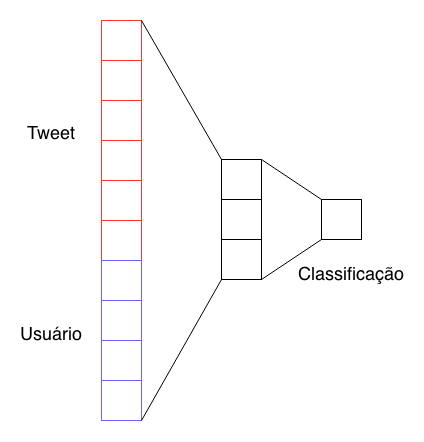
\includegraphics[scale=0.45]{images/network_composition.png}
    \caption{Representação da arquitetura multimodal composta pela combinação de
        classificadores de informação textual e de usuário concatenados.
        Em vermelho temos a representação da informação textual de um \textit{tweet}
        obtida pela camada de saída das redes CNN ou LSTM treinadas na etapa anterior,
        desconsiderando-se o neurônio de saída das redes.
        Em azul mostramos as representações do usuário autor do \textit{tweet} obtida
        pelos modelos de redes.
        A direita observamos as duas camadas \textit{feed-forward} responsáveis pela
        classificação.}
    \label{fig:network_composition}
    \end{center}
}
\end{center}
\end{figure}

  \chapter{Resultados e Discussões}
\label{chapter:results}

% BASE
% termos e temas coletados
% tabela de escolha de emoticons
% volume da base taggeada automaticamente
% relacao usuarios (retweets)
% status dos grafos
% volume da base de teste

A etapa de coleta de dados captou aproximadamente 9,2 milhões de tweets únicos
entre 2018 e 2019.
Parte desses tweets foi coletada da amostragem do conjunto total de mensagens
publicadas e outra parte da amostrada por dentre os tópicos: \textit{Libertadores,
ENEM, Amazônia} e \textit{Rock in Rio}.
Nessa base há aproximadamente 45 milhões de retweets, fornecendo a conexão entre
pessoas que será utilizada para montar a rede de usuários.

Para anotação automática foram identificados os emoticons mais frequentes da
base de dados e classificados manualmente entre positivos e negativos,
desconsiderando os neutros.
A Tabela~\ref{tab:emoticons} mostra as classes dos emoticons selecionados.
Com esse conjunto de emoticons 580 mil tweets foram anotados por supervisão
distante, dentre os quais 130 mil marcados como negativos e 450 mil marcados como
positivos.

\begin{table}[h]
    \begin{center}
        \begin{tabular}{| l | c |}
        \hline
        \textbf{Classe} & \textbf{Emoticons} \\ \hline
        Positiva &
            
\includegraphics[height=1em]{images/emojis/2764}
            
\includegraphics[height=1em]{images/emojis/1F602}
            %\includegraphics[height=1em]{images/emojis/1F5A4}
            %\includegraphics[height=1em]{images/emojis/1F923}
            
\includegraphics[height=1em]{images/emojis/1F60D}
            
\includegraphics[height=1em]{images/emojis/2665}
            %\includegraphics[height=1em]{images/emojis/1F970}
            
\includegraphics[height=1em]{images/emojis/1F605}
            
\includegraphics[height=1em]{images/emojis/1F601}
            %\includegraphics[height=1em]{images/emojis/1F92D}
            
\includegraphics[height=1em]{images/emojis/1F618}
            
\includegraphics[height=1em]{images/emojis/1F609}
            
\includegraphics[height=1em]{images/emojis/1F496}
            
\includegraphics[height=1em]{images/emojis/1F495}
            
\includegraphics[height=1em]{images/emojis/1F606}
            %\includegraphics[height=1em]{images/emojis/1F973}
            
\includegraphics[height=1em]{images/emojis/1F499}
            
\includegraphics[height=1em]{images/emojis/1F389}
            
\includegraphics[height=1em]{images/emojis/1F61D}
            
\includegraphics[height=1em]{images/emojis/1F49A}
            
\includegraphics[height=1em]{images/emojis/1F49C}
            %\includegraphics[height=1em]{images/emojis/2763}
            
\includegraphics[height=1em]{images/emojis/1F60A}
            
\includegraphics[height=1em]{images/emojis/1F60B}
            %\includegraphics[height=1em]{images/emojis/1F917}
        \\ \hline
        Negativa &
            
\includegraphics[height=1em]{images/emojis/1F62D}
            
\includegraphics[height=1em]{images/emojis/1F645}
            %\includegraphics[height=1em]{images/emojis/1F926}
            
\includegraphics[height=1em]{images/emojis/1F621}
            
\includegraphics[height=1em]{images/emojis/1F614}
            %\includegraphics[height=1em]{images/emojis/1F92C}
            %\includegraphics[height=1em]{images/emojis/1F92E}
            
\includegraphics[height=1em]{images/emojis/1F629}
            
\includegraphics[height=1em]{images/emojis/1F622}
            
\includegraphics[height=1em]{images/emojis/1F620}
            
\includegraphics[height=1em]{images/emojis/1F612}
            
\includegraphics[height=1em]{images/emojis/1F624}
            
\includegraphics[height=1em]{images/emojis/1F494}
            
\includegraphics[height=1em]{images/emojis/1F62A}
            
\includegraphics[height=1em]{images/emojis/1F625}
            
\includegraphics[height=1em]{images/emojis/1F62B}
            \includegraphics[height=1em]{images/emojis/1F630}
        \\ \hline
        \end{tabular}
        \caption{Emoticons selecionados para aplicação de supervisão distante.}
        \label{tab:emoticons}
    \end{center}
\end{table}

A rede de usuários foi formada por retweets entre usuários.
Os 45 milhões de retweets formam uma rede de 28 milhões de arestas únicas
conectando 5,5 milhões de vértices, representando uma densidade de
$9,4\mathrm{e}{-7}$.
O coeficiente de clusterização global é de $9,6\mathrm{e}{-4}$, portanto,
havendo um vizinho em comum o nó tem 1000 vezes mais chance de estar conectado a
outro nó do que quando ambos não compartilham conexões.
Aproximadamente 4,5\% dos nós pertencem a componente fortemente conexa, ou seja,
sub-grafo direcional em que existe um caminho entre todos os vértices.
Enquanto 97\% dos nós pertencem a componente fracamente conexa, que leva em
consideração o sub-grafo não direcional.
Observa-se que a rede inteira é formada praticamente por uma única componente
gigante enquanto os outros 3\% dos usuários estão distribuídos em um grande
volume de pequenas componentes.
A Figura~\ref{fig:graph_ccdf} mostra as distribuições de grau dos vértices.
Analisa-se que tanto a distribuição de grau de entrada quanto a de saída tem
caudas longas apesar da curva da distribuição de de grau de entrada ser
significativamente mais extensa.
Ressalta-se também que mais que 80\% dos nós tem grau de entrada 0, ou seja,
são usuários que não receberam nenhum retweet.
A Figura~\ref{fig:graph_distance} mostra a distância entre os nós da rede, que
tem média $8,8$.
Conclui-se portanto que dentre os dados captados formou-se uma rede com número
significativo de usuários e possuí características comumente observadas em redes
como a formação de \textit{hubs}, pequena distância média e grande componente
conexa.

\begin{figure}[h]
\begin{center} {
    \begin{center}
    \includegraphics[scale=0.65]{images/graph_ccdf.png}
    \caption{Gráfico da \textit{CCDF (complementary cumulative distribution function)}
             dos graus de entrada e saída da rede de usuários.
             O eixo horizontal representa o grau $k$ enquanto o eixo vertical
             demonstra a probabilidade de um vertice ter grau pelo menos $k$.}
    \label{fig:graph_ccdf}
    \end{center}
}
\end{center}
\end{figure}

\begin{figure}[h]
\begin{center} {
    \begin{center}
    \includegraphics[scale=0.65]{images/graph_distance.png}
    \caption{Distância entre pares de nós da rede de usuários.}
    \label{fig:graph_distance}
    \end{center}
}
\end{center}
\end{figure}

Uma vez finalizada a etapa de coleta dos dados, o processo de anotação e a
formação da rede de usuários, se prosseguiu para a etapa do classificador de
sentimento textuais.
Esses classificadores serão usados como base de comparação para avaliar a
eficiência dos classificadores multi-modais.

\section{Classificadores textuais não Neurais}

Os primeiros classificadores textuais treinados foram os por Naive Bayes e SVM.
Nesse caso, ambos usaram a representação Bag-of-Words.
O vocabulário formado a partir da base coletada é formado por um 127 mil
palavras.
O treinamento do algoritmo de Naive Bayes multinomial foi feito utilizando
validação cruzada por K-partições, no total de 10 partições, sob os dados de
treinamento anotados com supervisão distante. O parâmetro de suavização foi
escolhido por \textit{grid search}, de maneira a maximizar a área sob a curva ROC.
A Figura~\ref{fig:nb_grid} mostra a resposta do modelo para os diferentes fatores
de suavização testados.
O hiperparâmetro selecionado foi o de valor $0,244$, que obteve AUC de $0,862 \pm 0,002$.
Uma vez selecionado o melhor modelo na base de treino, o mesmo foi avaliado com
os dados da base de teste, que foram anotados manualmente.
A Figura~\ref{fig:nb_roc} apresenta a curva ROC dos dados de treino.
Observa-se que o mesmo modelo ao ser aplicado aos dados de teste tem resultado
de $0,801$ de área sob curva ROC.
Vê-se que há uma diferença de performance entre as diferentes bases, que
sobressaí a dispersão observada nas partições do treinamento.
% Este aspecto da supervisão distante será discutido no Capítulo~\ref{chapter:conclusion}.
% TODO: comentar mais pra frente, mas ainda nesse capitulo.
Concluindo a análise do modelo de Naive Bayes, utilizou-se os dados de treino
para encontrar o limiar de classificação que maximiza o índice SP.
O limiar encontrado teve o valor de $0,88$ e a Figura~\ref{fig:nb_confusion}
apresenta a matriz confusão correspondente a esse valor.
% TODO: comentar alto falso positivo?

\begin{figure}[h]
\begin{center} {
    \begin{center}
    \includegraphics[scale=0.65]{images/nb_grid.png}
    \caption{Resposta do modelo de Naive Bayes a variação do parâmetro de suavização.
             A linha cheia representa a média dos valores das 10 partições
             enquanto a área em azul, limitada pela linha rachurada, representa um desvio padrão.
             A linha vertical vermelha ressalta o paramêtro de maior média.}
    \label{fig:nb_grid}
    \end{center}
}
\end{center}
\end{figure}

\begin{figure}[h]
\begin{center} {
    \begin{center}
    \includegraphics[scale=0.65]{images/nb_roc.png}
    \caption{Curva ROC do modelo de Naive Bayes aplicado aos dados de teste.}
    \label{fig:nb_roc}
    \end{center}
}
\end{center}
\end{figure}

\begin{figure}[h]
\begin{center} {
    \begin{center}
    \includegraphics[scale=0.65]{images/nb_cm.png}
    \caption{Matrix confusão do modelo de Naive Bayes.}
    \label{fig:nb_confusion}
    \end{center}
}
\end{center}
\end{figure}

Em seguida, testou-se o classificador por SVM, modelo que obteve melhor
resultados nos testes feitos por \citet{go09}.
O vocabulário utilizado para codificação one-hot foi o mesmo aplicado ao
Naive Bayes.
Também se aplicou validação cruzada com 10 partições para determinar o melhor
parâmetro de regularização $L_2$.
A Figura~\ref{fig:svm_grid} apresenta os valores de AUC obtidos nos dados de
treino para o intervalo de parâmetro testado.
Observamos que o valor máximo obtido de AUC nos dados de treino foi
$0,904 \pm 0,001$, para o fator de regularização $7e^-05$.
Porém, ao aplicar o modelo aos dados de teste, a performance do modelo cai
consideravelmente, como vemos na Figura~\ref{fig:svm_roc}, com $0,647$ de área
da curva ROC.
O threashold de maior índice SP foi $0,776$, obtendo a matriz confusão
apresentada na Figura~\ref{fig:svm_confusion}.
A matriz confusão mostra que o model consegue distinguir elementos da classe
positiva, entretanto, ao ser aplicado em frases negativas o mesmo não conseguiu
performance melhor que escolha aleatória.
Observa-se também que apesar do modelo SVM superar as métricas do modelo de
Naive Bayes nos dados de treino, SVM generaliza significativamente menos quando
aplicado ao banco de dados de teste.
Apresentando assim uma grande discrepância entre a performance da base anotada
por supervisão distante e a classificada manualmente.

\begin{figure}[h]
\begin{center} {
    \begin{center}
    \includegraphics[scale=0.65]{images/svm_grid.png}
    \caption{Resposta do modelo de SVM a variação do parâmetro de regularização.
             A linha cheia representa a média dos valores das 10 partições
             enquanto a área em azul, limitada pela linha rachurada, representa um desvio padrão.
             A linha vertical vermelha ressalta o paramêtro de maior média.}
    \label{fig:svm_grid}
    \end{center}
}
\end{center}
\end{figure}

\begin{figure}[h]
\begin{center} {
    \begin{center}
    \includegraphics[scale=0.65]{images/svm_roc.png}
    \caption{Curva ROC do modelo de SVM aplicado aos dados de teste.}
    \label{fig:svm_roc}
    \end{center}
}
\end{center}
\end{figure}

\begin{figure}[h]
\begin{center} {
    \begin{center}
    \includegraphics[scale=0.65]{images/svm_cm.png}
    \caption{Matrix confusão do modelo de SVM.}
    \label{fig:svm_confusion}
    \end{center}
}
\end{center}
\end{figure}


% emoticon sarcastico?

\section{Classificadores textuais por Redes Neurais}

Proseguindo para os classificadores por redes neurais, começamos com o
treinamento da representação de texto.
Realizou-se o treino do \textit{Word2Vec} com os parâmetros
apresentados na Seção~\ref{sec:nlp-classifier}.
O treinamento foi executado até a convergência da função custo.

Obtido o modelo \textit{Word2Vec}, foi realizado o treino dos classificadores de
redes neurais convolucionais.
Algumas das curvas de treinamento são demonstradas na Figura~\ref{fig:cnn_train}.
Observamos que, normalmente, após a terceira época a função custo de treinamento
apresenta uma estabilidade.
Devido ao \textit{early stopping} cada treinamento acaba em épocas diferentes.
Como aplicamos \textit{dropout} e regularização durante o treinamento temos que
a entropia cruzada de treinamento é mais alta do que a de validação.
Ressaltamos que os treinamentos convergiram para valores parecidos, não
oscilando entre diferentes mínimos locais.

Seguimos com o treinamento do modelo de LSTM, mantendo a entrada com a
representação \textit{Word2Vec}.
A Figura~\ref{fig:lstm_train} apresenta uma amostra dos 10 treinamentos
realizados da rede LSTM.
Vemos que com LSTM demorou-se mais para atingir convergência, sendo precisas
30 a 50 épocas de treino até a estabilização da função custo.
Observamos também que assim como as redes convolucionais, não houve grande
variação entre os mínimos encontrados pelas diferentes realizações de
treinamento das redes.

Finalmente, utilizaremos o ELMo como forma de representação em conjunto com o
classificador de redes convolucionais.
O alto custo computacional de treinamento desse modelo implicou em algumas
limitações de sua execução.
Obtive-se pesos pré-treinados, portanto, não pode se selecionar a
dimensionalidade da representação.
Neste caso, cada palavra será representada por um vetor de tamanho $1024$.
Também não foi possível fazer múltiplas realizações do treinamento.
A rede convolucional, responsável pela classificação, foi treinada com os mesmos
hiper-parâmetros adotados em sua versão com entrada por \textit{Word2Vec}.
A Figura~\ref{fig:elmo_train} apresenta a curva de treinamento do modelo.

% val loss < train loss pq train tem validacao
% https://twitter.com/aureliengeron/status/1110839223878184960

\begin{figure}[h]
\begin{center} {
    \begin{center}
    \includegraphics[scale=0.25]{images/cnn_train.png}
    \caption{Curvas de treinamento de classificadores por redes neurais
        convolucionais.}
    \label{fig:cnn_train}
    \end{center}
}
\end{center}
\end{figure}

\begin{figure}[h]
\begin{center} {
    \begin{center}
    \includegraphics[scale=0.25]{images/lstm_train.png}
    \caption{Curvas de treinamento de classificadores por redes neurais LSTM.}
    \label{fig:lstm_train}
    \end{center}
}
\end{center}
\end{figure}

\begin{figure}[h]
\begin{center} {
    \begin{center}
    \includegraphics[scale=0.45]{images/elmo_cnn_train.png}
    \caption{Curvas de treinamento do modelo com representação ELMo e classificador de CNN.}
    \label{fig:elmo_train}
    \end{center}
}
\end{center}
\end{figure}

\section{Classificadores Multimodais}

Seguimos para a incorporação da informação dos grafos de usuários nos modelos.
Como descrito na seção \ref{sec:multimodal-classifier}, o grafo foi reduzido a
sua componente principal para reduzir os requisitos de memória necessários para
o treinamento dos modelos.
O aprendizado foi realizado em duas etapas: aquisição de \textit{embeddings} a
partir de modelagem não-supervisionada do grafo; posteriormente foi realizado o
treinamento em conjunto com os modelos textuais treinados na anteriormente.

As redes conjuntas compostas pelas camadas concatenadas da representação textual
do \textit{tweet} com a representação do grafo do usuário, seguida de 2 camadas
classificatórias de tamanhos repectivamente de $100$ e $32$ neurônios completamente
conectados.
Os pesos das representações do usuário e textuais continuaram a sofrer
\textit{fine-tunning} durante a otimização do modelo.
Assim como nos classificadores textuais, a seleção do \textit{threshold} de
classificação foi definida pelo ponto de maximização do índice SP.

Começando pelo treinamento da representação por \textit{Locally Linear Embedding}.
Pelo algoritmo depender da matriz de adjacência, que tem custo quadrático em
memória, foi necessário limitar o número de usuários da rede.
Foram selecionados aleatóriamente $10$ mil usuários dentro da sub-grafo de
usuários da maior componente conectada para o treinamento do algoritmo.
Foram feitas $10$ realizações do treinamento, cada uma com seu próprio conjunto
de nós selecionados.
O modelo foi treinado para extrair uma representação de dimensão $128$.
Para melhor comparar os diferentes métodos esse número será mantido pelos outros
métodos.
Os usuários que não foram selecionados no sorteio do treinamento tiveram sua
representação no vetor zero.

Posteriormente foram treinados o algoritmo \textit{Node2Vec}.
Mantiveram-se as $10$ realizações do treinamento e o tamanho do vetor de
representação.
Como este algoritmo não depende da matriz de adjacência, foram realizados os
treinamentos considerando todos os usuários presentes na maior componente.
Neste algoritmo consideramos o grafo como não-direcionado e removemos as arestas
de um nó a si mesmo.
Os parâmetros de treinamento do algoritmo foram baseados no proposto por
\citet{grover16}.
Os valores de parâmetro $p$ e $q$ de amostragem foram definidos em $1$.
Os passeios aleatórios para definição dos contextos tiveram $80$ passos
de interação e foram feitas $10$ realizações de passeio por vértice.
Os pesos das arestas não foram considerados durante a realização dos passeios
aleatórios.
Utilizou-se janelas de contexto de tamanho $10$ e treinou-se a otimização dos
pesos por $3$ épocas.

Por fim, treinou-se a rede convolucional de grafos (GCN).
Assim como no caso do \textit{Node2Vec} também se utilizou todo o subgrafo
presente na principal componente.
Assim como nos modelos anteriores continou-se com as $10$ inicializações e o
tamanho da representação dos nós em $128$ dimensões.
Pelo GCN depender de atributos do vértices para o treinamento da representação,
utilizou-se um atributo obtido pelo próprio grafo, o log do graú do nó.
Essa escolha se deu pois não necessita de extrações adicionais de dados.
Outros atributos dos usuários poderiam ter sido incorporados caso houvesse a
disponibilidade desses dados como: número de seguidores, localização,
frequência de uso, etc.
O modelo foi treinado até a finalização por \textit{early stopping}.

% TODO: matrix confusao dos modelos neurais? ou grafico de distribuicao das
% predicoes

Concluimos os experimentos com a Figura~\ref{fig:experiment_results}
consolidando os resultados obtidos por todos experimentos.
Há diversas análises há serem feitas a partir destes resultados.
Primeiramente, observamos que ao contrario do que esperavamos baseados nos
trabalhos referenciados no Capítulo~\ref{chapter:nlp}, entre os modelos
puramente textuais vemos que os baseados em redes neurais obtiveram resultados
piores que as técnicas tradicionais SVM e Naive Bayes.
Há diferentes hípoteses que podem ser responsáveis por essas diferença.
A representação de palavras avaliadas nos classificadores neurais,
\textit{Word2Vec} e \textit{ELMo}, podem não ter conseguido obter boas
transformações necessárias para a discriminação entre as classes.
Apesar do modelo \textit{Word2Vec} ter se provado eficiente na captação de
contexto sintático e semântico, a grande maioria dos estudos analisados utilizam
textos em formatos longos como artigos jornalistico.
Há também a possiblidade de que a base de \textit{tweets} disponivel para o seu
treinamento não tenha sido suficiente para o modelo adquirir estatística
suficiente dos dados.
A representação pelo modelo \textit{ELMo}, por sua vez, foi treinada com artigos
da Wikipedia.
A diferença de linguagem entre esse meio e as redes sociais pode ser um dos
fatores responsáveis pela não reprodução dos bons resultados da técnica nesta
base de dados.
A vantagem das técnicas de classificacao menos complexas pode demonstrar ainda
uma dificuldade no treinamento de dados provindos de textos curtos e informais
ou a necessidade de volumes maiores de dados de treinamento do que os coletados
para esse experimento.

Observa-se também que adicionar informações do usuário apresentou resultados
variados.

Continuando a analise, A supervisao distante... pode ter problema no positivo.. vide matrix confusao...


% diferente do esperado nlp
% diferente do esperado mixed
% faltou base de treino?
% nao funciona bem em texto curto e informal
% supervised sendo ruim pra modelos complexos?
% problema so nos positivos, pode ser a selecao de emoticon
% problema na representacao de palavras? w2v e elmo
% retweet nao representando bem o usuario?
% TODO: comentar alta taxa de falso positivo do modelo e como isso pode ser consequencia do treinamento semi supervisionado

\begin{figure}[h]
\begin{center} {
    \begin{center}
    \includegraphics[scale=0.35]{images/experiment_results.png}
    \caption{Comparativo entre modelos textuais e multimodais apresentados nesse
             trabalho. A figura apresenta a área sob a curva ROC dos modelos
             avaliados quando aplicados aos dados de teste.}
    \label{fig:experiment_results}
    \end{center}
}
\end{center}
\end{figure}

% FIZ UM BACKUP DE MODELS E JOGUEI EM /mnt/models

  \chapter{Conclusões}


  \backmatter
  \bibliographystyle{coppe-unsrt}
  \bibliography{thesis}

  \appendix
  %\chapter{Algumas Demonstra{\c c}\~oes}

\end{document}
